\documentclass[oneside]{book}

\title{MIPS Home Computer System}
%\subtitle{System Design Reference}
\author{
    \large Student\\
    \large Mostafa Abd El-Aziz\\
    \and
    \large Supervisor\\
    \large Prof. Dr. Layla Abou Hadid\\
}
\date{\vspace{-5ex}}

% font
\usepackage[T1]{fontenc}
\usepackage{lmodern}
\renewcommand*\familydefault{clms}
\usepackage{sfmath}
\usepackage{microtype}
\usepackage[utf8]{inputenc}
\usepackage{cfr-lm} % font package
\usepackage{scrextend}
\changefontsizes{12pt}
\usepackage{inconsolata}

% listings
\usepackage{listings}
\lstset{language=java}

% margins
\usepackage[margin=3cm,a4paper]{geometry}

% figures and tables
\usepackage{graphicx}
\usepackage{float}
\usepackage{multirow}
\usepackage{tikz}
\usepackage{colortbl}
\usepackage{xcolor}

% table of contents
\usepackage{tocloft}
\renewcommand{\cftsecleader}{\cftdotfill{\cftdotsep}} % for chapters
\renewcommand{\cftpartleader}{\cftdotfill{\cftdotsep}} % for parts
\setcounter{tocdepth}{5}

% section style
\usepackage{enumitem}
\usepackage{sectsty}
\sectionfont{\LARGE}
\setcounter{secnumdepth}{5}

% page orientation
\usepackage{lscape}

% title page
\usepackage[eng,exjobb]{KTHEEtitlepage}

% navigation window
\usepackage{hyperref}
\hypersetup{pdftex,colorlinks=true,allcolors=blue}
\usepackage{hypcap}

% verbatim
\usepackage{fancyvrb}

%------------------------------------------------------------------------------%

\begin{document}

\frontmatter

%------------------------------------------------------------------------------%

\ititle{MIPS Computer System on FPGA}
%\isubtitle{My Subtitle} % Optional
\idate{July 2016}
\iauthor{Mostafa Abd El-Aziz}
\makeititle

%------------------------------------------------------------------------------%

\newpage
\thispagestyle{plain}
\chapter{Abstract}

%------------------------------------------------------------------------------%

\newpage
\thispagestyle{plain}
\chapter{Acknowledgements}

%------------------------------------------------------------------------------%

\newpage
\thispagestyle{plain}
\topskip0pt
\vspace*{\fill}
\bfseries
\begin{Verbatim}[showspaces=false,fontsize=\small]
                     ,----------------,              ,---------,
                ,-----------------------,          ,"        ,"|
              ,"                      ,"|        ,"        ,"  |
             +-----------------------+  |      ,"        ,"    |
             |  .-----------------.  |  |     +---------+      |
             |  |                 |  |  |     | -==----'|      |
             |  |  WE LOVE MIPS   |  |  |     |         |      |
             |  |  QUAF> _        |  |  |/----|`---=    |      |
             |  |                 |  |  |   ,/|==== ooo |      ;
             |  |                 |  |  |  // |(((( [33]|    ,"
             |  `-----------------'  |," .;'| |((((     |  ,"
             +-----------------------+  ;;  | |         |,"
                /_)______________(_/  //'   | +---------+
           ___________________________/___  `,
          /  oooooooooooooooo  .o.  oooo /,   \,"-----------
         / ==ooooooooooooooo==.o.  ooo= //   ,`\--{)B     ,"
        /_==__==========__==_ooo__ooo=_/'   /___________,"
        `-----------------------------'
\end{Verbatim}
\normalfont
\vspace*{\fill}

%------------------------------------------------------------------------------%

\newpage
\renewcommand{\contentsname}{Contents}
\tableofcontents

%------------------------------------------------------------------------------%

\newpage
\listoffigures

%------------------------------------------------------------------------------%

\mainmatter

%------------------------------------------------------------------------------%

{\let\clearpage\relax \chapter{Introduction}}

The past few years have witnessed great development in the area of
field programmable gate array (FPGA) devices. The high flexibility and
performance of FPGAs make them a suitable choice for systems with
high constraints. The main purpose of our project is to build a simple
computer system using a cheap FPGA device. \\

\section{Overview}

In this project we shall use FPGA technology to implement a general-purpose
computer machine based on MIPS-I instruction set architecture. We define the
term `general-purpose computer' as a computer that should be able to
perform most common computing tasks, like editing documents, performing
calculations, and programming.\\

The system consists of several components, like CPU, memory, input devices,
and output devices, all connected together to build up a general-purpose
computer. The hardware part of the machine is implemented using the FPGA
chip. The software part is a set of programs stored in the memory of
the system.\\

The CPU is an implementation for MIPS-I instruction set architecture with
a 5-stage pipeline. CPU, along with other hardware components, is implemented
in VHDL (VHSIC Hardware Description Language) while software is written
in MIPS assembly and C programming language. There is also an emulator
for the machine written in C language for GNU/Linux.\\

Figure \ref{computer} shows the basic conception of the proposed system.
The system has a CRT/LCD screen used to output information to the user,
and a keyboard used for input. Power is regulated using an AT-compatible
power supply. The FPGA board contains an FPGA chip, which is automatically
configured with our hardware design on start up.\\

The FPGA board also contains other components, including a ROM chip,
a RAM chip, LEDs, switches, VGA connector, and a PS/2 keyboard connector.
Our hardware design (that lies inside the FPGA chip) is responsible for
interfacing all these components. The software part of our machine
is stored on the ROM chip.

\begin{figure}[H]
\begin{center}
\includegraphics[width=0.9\textwidth]{computer.png}
\end{center}
\caption{Overview of the computer system}
\label{computer}
\end{figure}

The system actually consists of several layers: hardware, firmware, and
software. User interacts with applications that runs over the operating
system. Figure \ref{layers} shows the layered architecture of the system.

\begin{figure}[H]
\begin{center}
\includegraphics[width=0.55\textwidth]{layers.png}
\end{center}
\caption{System layers}
\label{layers}
\end{figure}

When the computer boots up, CPU starts executing firmware instructions that
are stored on the ROM chip on the board. Firmware initializes the hardware
components and loads the operating system into RAM. The OS boots up
the machine and provides a user-friendly interface to the end user.

\section{Scope of Project}

As we mentioned in the overview section, the goal of this project is to build a
general-purpose computer system based on MIPS architecture
using FPGA technology. Users shall communicate with the system using
a command-line interface. Since the machine is `programmable', in the
sense that end user can write programs, compile, and execute them, the machine
can be used for any purpose. However, because the resources of the FPGA are
very limited, the machine doesn't have a graphical user interface.

\section{Overview of Document}

In this document, we describe the architecture and the implementation
of the proposed computer system in details. First, we shall define two
keywords that will be used throughout the document:

\begin{itemize}

\item \textbf{Architecture}:
     The behaviour of the processor as seen by the programmer.
     This includes the instruction set, their opcodes and formats,
     architectural registers, interrupt/exception protocols, and other
     behavioral concerns that will be seen later in the section.
     The architecture describes all that can be abstracted from the
     implementation of the processor. Other authors may call this an
     instruction set architecture (ISA) or macro-architecture.

\item \textbf{Micro-architecture}:
     How the architecture of the processor is implemented
     in switching circuits. We use this keyword to refer to our VHDL
     implementation for the architecture described in this section. There
     may exist several different implementations for the same architecture.
     The only restriction on the micro-architecture of a processor is to
     behave exactly as described by the architecture, but the implementation
     itself doesn't matter. For example, the architecture might guarantee
     that the 'effect' of the execution of a set of instructions will be
     in order, however, the processor might execute the instructions in an
     out of order fashion (OoOE) yet effectively behaves the same as
     described by the architecture.

\end{itemize}

We use the word `architecture' to refer to the architecture of the processor
and the whole system. On the other hand, the word `implementation' is used
to refer to the micro-architecture of the processor and the whole system.
Indeed, there are two implementations for the system: one using FPGA,
and the other is emulator software.\\

The book is organized in chapters, summarized in the following lines:

\begin{itemize}

\item \textbf{Architecture}: Explains the architecture of the whole system,
and the architecture of system components, including CPU, system bus,
memory, and I/O devices.

\item \textbf{Implementation}: Describes how the architecture is implemented
on FPGA using VHDL language.

\item \textbf{Software}: Shows the architecture of the firmware and the
operating system.

\item \textbf{Results}: Screenshots and sample runs for the system.

\item \textbf{Conclusion}: Brief conclusion for our work and suggestions for
future work.

\end{itemize}

%------------------------------------------------------------------------------%

\chapter{Related Work}

%------------------------------------------------------------------------------%

\chapter{Architecture}

In this chapter we introduce the high-level design of the machine
we propose in this project. We use the word `architecture' to refer
to the programming model of the machine (the design of the machine as
seen by the programmer), as we've already explained in chapter 1.\\

First, we will show the major \textit{architectural} components of the
system. Next, we describe every component
in a separate section. We refer to our machine using the word `system',
since it can be seen as a set of interacting components whose behaviour can be
described using black box model. This chapter is dedicated for getting
into this black box; in order to explore the architecture (the behaviour
and the interface) of every component by itself.

\section{Top-Level Components}

Similar to the majority of modern digital computers, our computer consists
of a centeral processing unit, connected to memory and I/O devices
through system bus. The I/O devices include a circuit for interfacing
PS/2 keyboard (called keyboard controller), a programmable timer,
interrupt controller, and a video graphics adapter (VGA) component.\\

\begin{figure}[h]
\begin{center}
\includegraphics[width=0.9\textwidth]{toplevel.png}
\end{center}
\caption{Top-level components of the system.}
\label{toplevel}
\end{figure}

Figure \ref{toplevel} shows the architectural components of the system
(yet it hides many details). The components are summarized in the
following points:

\begin{itemize}

\item \textbf{Central Processing Unit (CPU)}:
The CPU is actually the bus master. It has the capability of
driving the system bus at any time. CPU fetches/writes data from/to
memory and I/O devices through system bus. When CPU needs to access
a word in memory (or an I/O device), CPU puts the address corresponding
to the word in memory or the target I/O device on address bus. The device
shall respond to the access request by reading/writing data from/to data
bus.

\item \textbf{System Bus}:
The bus through which all components of the system are connected. The bus
consists of three sub-buses:

\begin{itemize}

\item Address bus (32 lines): always driven by the CPU. Contains the address
of the data word being read/written by CPU.

\item Data bus (32 lines): holds the data during an access cycle.

\item Control bus: set of control signals controlled by the processor and
address decoder during an access cycle.

\end{itemize}

\item \textbf{Bus Decoder}:

This component keeps listening to the address bus to control which device
should respond to read/write request issued by CPU. The decoder takes
the most significant bits of the address as input, and controls a number
of chip select (CS) signals for all I/O devices in the system. A device
whose CS signal is active is the one that should respond to CPU.

\item \textbf{Memory Interface}:

This is a circuit that works as an interface between our system and a CMOS
pseduo-static 16MB RAM chip used as main memory. Another ROM chip is also
connected to the back side of the circuit. The circuit can be considered as
a translation between the language of our system bus and the pinout
of the memory chips.

\item \textbf{VGA Interface}:

This is an interface between our system and a VGA-compatible connector.
It is used to provide a method of displaying text data on a CRT/LCD screen
that supports VGA interface.

\item \textbf{Interrupt Controller}:

Provides a protocol for interrupting the processor by various I/O devices.
Several interrupt lines are fed into the interrupt controller. The output
of the controller is an interrupt signal that is delivered to the processor.
When interrupt service routine (ISR) is executed, software should ask
the interrupt controller for more information about the interrupt source.

\item \textbf{Programmable Interval Timer}:

Used by the operating system to keep track of the time of day. Can be
programmed to trigger an interrupt every specific interval configured
by the OS. Details of the architecture of the interval timer will be
seen later in this chapter.

\item \textbf{Keyboard Controller}:

Provides an interface between the system and an external PS/2 keyboard
that is used as an input device. It is also connected to the interrupt
controller through an interrupt signal (to interrupt the CPU whenever
a key is pressed down).

\end{itemize}

\section{Central Processing Unit}

The CPU module implements MIPS-I instruction set architecture along with
additional instructions that control the behavior of the processor. In this
section we present detailed description for the programming interface
of the CPU, followed by a description for the implementation of that
interface.

\subsection{Introduction}

CPU instruction (also called order, operation) is the basic unit
of execution. The main task of a processor is to execute a sequence
of instructions (i.e, program) which shall have effect on the state
of the processor and devices connected with the processor.\\

Following Von Neumann's model, the program is stored in memory along
with variables which are accessible and modifiable by the program.
Memory is an array of words, where a word in MIPS is 32 bits. Every
instruction in MIPS is encoded in a single word that contains
the opcode and the operands of the instruction.\\

Every word in memory has an address, that also means that every
instruction in memory has an address called `instruction address'.
CPU maintains a register that stores the instruction address of
next instruction to fetch, called program counter (PC). When an
instruction is fetched, program counter is increased by 4 (number
of bytes in word) without touching lower 2 bits (they are
always zero), a behaviour which implies that:

\begin{itemize}

\item Unless there is a branch, a jump, or an exception, instructions
      are always executed in sequence, as opposed to machines with
      one-plus-one addressing scheme like RPC-4000 where a program
      could be scattered over the drum.

\item Instructions should always be stored in 4-byte aligned words.

\end{itemize}

It is important to note that MIPS-I instruction set is a proper
subset of the instruction set of our processor; meaning that
the processor supports additional instructions and registers that
control the behaviour of the processor as will be seen below.\\

CPU instructions are divided into the following groups:

\begin{enumerate}

\item Load and Store
\item ALU
\item Jump and Branch
\item Miscellaneous
\item Control

\end{enumerate}

\subsubsection{Load and Store Instructions}

This group holds all instructions related to memory access, either
read/load or write/store accesses. Every instruction word contains
the following fields:

\begin{itemize}

\item \textbf{Opcode}: specifies that this instruction is a memory
                       instruction, along with whether this instruction
                       is a byte, half-word, or a word instruction, and
                       whether this instruction is an aligned/unaligned,
                       load/store, and signed/unsigned instruction
                       (6 bits).

\item \textbf{Source/destination register}: If the instruction is a load
                                            instruction, this is the address
                                            of the register where the value
                                            loaded from memory will be stored.
                                            If the instruction is a store
                                            instruction, this is the address
                                            of the register where the value
                                            stored to memory will be loaded.
                                            Since there are 32 data registers
                                            specified by MIPS ISA, this field
                                            takes a value from 0 to 31
                                            (5 bits).

\item \textbf{Base register}: address of data register that contains
                              the base memory address. Just like
                              source/destination register field, this
                              field takes a value from 0 to 31 (5 bits).

\item \textbf{Index immediate}: A 16-bit signed integer that is extended to
                                32-bit signed integer then added to the value
                                of the base register. Result is the memory
                                address that will be accessed.

\end{itemize}

This instruction group has a total of 12 instructions, each instruction
has a unique value for the opcode field:

\begin{enumerate}

\item \textbf{LB}:  Load Byte
\item \textbf{LBU}: Load Byte Unsigned
\item \textbf{SB}:  Store Byte
\item \textbf{LH}:  Load Halfword
\item \textbf{LHU}: Load Halfword Unsigned
\item \textbf{SH}:  Store Halfword
\item \textbf{LW}:  Load Word
\item \textbf{SW}:  Store Word
\item \textbf{LWL}: Load Word Left
\item \textbf{LWR}: Load Word Right
\item \textbf{SWL}: Store Word Left
\item \textbf{SWR}: Store Word Right

\end{enumerate}

The detailed behaviour of those instructions is described
in the appendix.\\

As described above, the target memory address is calculated by
adding the extended 32-bit signed immediate to the value of
the base register, forming a 32-bit memory address. This implies
that memory address space of MIPS-I instruction set is 4GB. There
are two characteristics that apply to the address field:

\begin{itemize}

\item \textbf{Alignment}: All instructions (except LWL, LWR, SWL,
                          and SWR) are aligned. This means that
                          LW and SW target address must be
                          a multiple of 4, while LH, LHU, and
                          SH target address must be a multiple of 2.

\item \textbf{Endianness}: Our processor is little endian; the least
                           significant byte of a word in memory is the
                           byte having the lowest address, and the
                           most significant byte is the byte having
                           the highest address.

\end{itemize}

\subsubsection{ALU Instructions}

This group contains all instructions related to arithmetic
and logical operations. We divide them into 4 categories,
according to how they are encoded:

\begin{enumerate}

\item ALU instructions with an immediate operand
\item ALU instructions with three operands
\item Shift instructions
\item Multiply and divide instructions.

\end{enumerate}

We call the last three groups together as `R-TYPE ALU instructions'
for reasons illustrated below. In the next lines we describe the
instruction groups in detail.

\begin{itemize}
\item

\textbf{\underline{ALU Instructions With Immediate Operand:}} \\

The reader may expect that the first group (ALU instructions
with immediate operand) is encoded exactly the same way as
memory instructions. Both groups are included in the same
encoding class (called I-TYPE) as will be seen later in
the encoding subsubsection. Just like memory instructions,
an ALU instruction with an immediate operand shall consist
of the following fields:

\begin{itemize}

\item \textbf{Opcode}: specifies that this instruction is an ALU
                       with immediate operand instruction, along
                       with the type of operation. (6 bits)

\item \textbf{Source register}: except for LUI, all operations in
                                this group are binary operations, thus
                                this field contains the address of the
                                register that contains the value of
                                the first parameter of the binary
                                operation. For LUI instruction, this
                                field must be zero. (5 bits)

\item \textbf{Destination register}: address of data register where
                                     the result of the operation will
                                     be stored. (5 bits)

\item \textbf{Index immediate}: except for ANDI, ORI, XORI, and LUI
                                instructions, this field is a 16-bit signed
                                integer that is extended to 32-bit signed
                                integer then used as the second parameter
                                for the binary operation. For ANDI, ORI,
                                and XORI, this field is a 16-bit unsigned
                                integer that is extended to 32-bit unsigned
                                integer then used as the second parameter
                                for the binary operation. For LUI, this
                                field is just copied into the highest 16 bits
                                of the destination register.

\end{itemize}

Following is a listing for all ALU with immediate operand instructions
specified by MIPS-I ISA, with every instruction having a unique value
for the opcode field:

\begin{enumerate}

\item \textbf{ADDI}:  Add Immediate Word
\item \textbf{ADDIU}: Add Immediate Unsigned Word
\item \textbf{SLTI}:  Set on Less Than Immediate
\item \textbf{SLTIU}: Set on Less Than Immediate Unsigned
\item \textbf{ANDI}:  And Immediate
\item \textbf{ORI}:   Or Immediate
\item \textbf{XORI}:  Exclusive Or Immediate
\item \textbf{LUI}:   Load Upper Immediate

\end{enumerate}

The detailed behaviour of those instructions is described
in the appendix.\\

\item \textbf{\underline{R-TYPE ALU Instructions:}} \\

The remaining three groups of ALU instructions (ALU instructions
with three operands, shift instructions, and multiply/divide
instructions) are all encoded the same way which is shown below.
All instructions encoded that way are called R-TYPE instructions.
We will summarize all encoding classes later in this section.\\

\begin{itemize}

\item \textbf{Opcode}: always zero. (6 bits)

\item \textbf{Source register 1}: except for SLL, SRL, SRA, SLLV, SRLV,
                                  SRAV, MFHI, MTHI,
                                  MFLO, and MTLO instructions, this field
                                  contains the address of the register
                                  that holds the value of the first
                                  parameter for the binary operation.
                                  For SLLV, SRLV, and SRAV, this field
                                  contains the address of the register
                                  that holds the amount of shift.
                                  For SLL, SRL, SRA, MFHI, and MFLO
                                  instructions, this field must be zero.
                                  For MTHI and MTLO instructions, this
                                  field contains the address of the
                                  register that holds the value that
                                  will be moved into the HI/LO register.
                                  (5 bits)

\item \textbf{Source register 2}: except for SLL, SRL, SRA, SLLV, SRLV,
                                  SRAV, MFHI, MTHI, MFLO, and MTLO
                                  instructions, this field contains
                                  the address of the register that
                                  holds the value of the second parameter
                                  for the binary operation.
                                  For SLL, SRL, SRA, SLLV, SRLV, and
                                  SRAV instructions, this field contains
                                  the address of the register that
                                  holds the value to be shifted.
                                  For MFHI, MTHI, MFLO, and MTLO instructions,
                                  this field must be zero. (5 bits).

\item \textbf{Destination register}: except for MULT, MULTU, DIV, DIVU,
                                     MFHI, MTHI, MFLO, and MTLO instructions,
                                     this field contains the address of the
                                     data register where the result of the
                                     binary operation or shift operation will
                                     be stored.
                                     For MFHI and MFLO instructions, value
                                     stored in LO/HI register will be moved
                                     into the register addressed by this field.
                                     For MULT, MULTU, DIV, DIVU, MTHI, and MTLO
                                     instructions, this field must be zero,
                                     since the result of these instructions
                                     is stored directly in LO register, HI
                                     register, or both. (5 bits)

\item \textbf{Shift amount}: for SLL, SRL, and SRA instructions, this field
                             simply contains the amount of shift. For all
                             other instructions, this field must be zero.
                             (5 bits)

\item \textbf{Function code}: An extension to the opcode field, contains
                              a unique code that defines the instruction
                              to be performed. (6 bits).
\end{itemize}

With a unique function code for every instruction (and an opcode of 0),
ALU instructions with 3 operands group includes the following instructions:

\begin{enumerate}

\item \textbf{ADD}:  Add Word
\item \textbf{ADDU}: Add Unsigned Word
\item \textbf{SUB}:  Subtract Word
\item \textbf{SUBU}: Subtract Unsigned Word
\item \textbf{SLT}:  Set on Less Than
\item \textbf{SLTU}: Set on Less Than Unsigned
\item \textbf{AND}:  And operation
\item \textbf{OR}:   Or operation
\item \textbf{XOR}:  Exclusive Or operation
\item \textbf{NOR}:  Nor operation

\end{enumerate}

The third group (shift instructions) contains the following instructions:

\begin{enumerate}

\item \textbf{SLL}:  Shift Word Left Logical
\item \textbf{SRL}:  Shift Word Right Logical
\item \textbf{SRA}:  Shift Word Right Arithmetic
\item \textbf{SLLV}: Shift Word Left Logical Variable
\item \textbf{SRLV}: Shift Word Right Logical Variable
\item \textbf{SRAV}: Shift Word Right Arithmetic Variable

\end{enumerate}

Finally, following is a listing for all instructions in the last
group (multiply/divide instructions):

\begin{enumerate}

\item \textbf{MULT}:  Multiply Word
\item \textbf{MULTU}: Multiply Unsigned Word
\item \textbf{DIV}:   Divide Word
\item \textbf{DIVU}:  Divide Unsigned Word
\item \textbf{MFHI}:  Move From HI
\item \textbf{MTHI}:  Move To HI
\item \textbf{MFLO}:  Move From LO
\item \textbf{MTLO}:  Move To LO

\end{enumerate}

For detailed description for the behaviour of all of the instructions listed
above, please refer to the appendix.

\end{itemize}

\subsubsection{Jump and Branch Instructions}

MIPS-I architecture defines a number of operations that control the path
of execution. Jump instruction shall unconditionally modify PC register,
while branch instructions modify PC register only when the condition
specified within the instruction word is tautology.\\

Jump and branch instructions are divided into four groups:

\begin{enumerate}

\item Jump Instructions Jumping Within a 256MB Region
\item Jump Instructions to Absolute Address
\item PC-Relative Conditional Branch Instructions Comparing 2 Registers
\item PC-Relative Conditional Branch Instructions Comparing Against Zero

\end{enumerate}

Next we illustrate every group in detail.

\begin{itemize}

\item \textbf{\underline{Jump Instructions Jumping Within 256MB Region:}} \\

The way the instructions of the first group (jump instructions jumping
within 256MB region) are encoded is different from I-TYPE and R-TYPE. It's
called J-TYPE and consists of the following fields:

\begin{itemize}

\item \textbf{Opcode}: specifies that the instruction is a jump instruction
                       of J-TYPE, along with whether the instruction
                       should alter the link register or not. (6 bits)

\item \textbf{Instruction Index}: a 26-bit integer that is multiplied by 4
                                  to form the lowest 28-bit of the new value
                                  of PC register. The highest 4 bits are taken
                                  from the old value of PC, that's why the
                                  instructions of this group are said to
                                  jump within 256MB region (4GB/16).

\end{itemize}

This group only contains two instructions:

\begin{enumerate}

\item \textbf{J}:   Jump
\item \textbf{JAL}: Jump and Link

\end{enumerate}

\item \textbf{\underline{Jump Instructions to Absolute Address:}} \\

Second group (jump instructions to absolute address) consists of instructions
similar to instructions of the first group, yet have the ability to jump
to any memory location, not just locations inside the current 256MB region.
These instructions are encoded as R-TYPE like most ALU instructions, thus
the instruction word shall consist of the following fields:

\begin{itemize}

\item \textbf{Opcode}: always zero. (6 bits)

\item \textbf{Source register 1}: contains address of the register that
                                  holds the target 32-bit address. (5 bits)

\item \textbf{Source register 2}: must be zero. (5 bits)

\item \textbf{Destination register}: for JALR instruction, this field
                                     contains the address of the register
                                     where return address shall be stored.
                                     For JAL instruction, this field should
                                     be zero.

\item \textbf{Shift amount}: must be zero. (5 bits)

\item \textbf{Function code}: An extension to the opcode field, contains
                              a unique code that defines the instruction
                              to be performed (only jump or jump with
                              link). (6 bits).
\end{itemize}

Analogous to the first group, this group consists of these two instructions:

\begin{enumerate}

\item \textbf{JR}:   Jump Register
\item \textbf{JALR}: Jump and Link Register

\end{enumerate}

\item \textbf{\underline{Conditional Branch Instructions
                         Comparing 2 Registers:}} \\

The remaining two groups are concerned with conditional branching. The
third group consists of instructions that compare two registers, then
jump if the comparison yields a specific result, while the last
group compare one register against zero, and jump if the comparison
yields a specific result.\\

The third group is just encoded as I-TYPE (like ALU immediate
instructions and load/store instructions). The fields of the instruction
word are interpreted as following:

\begin{itemize}

\item \textbf{Opcode}: specifies that this instruction is a conditional
                       branch instruction comparing 2 registers, along
                       with the type of comparison to be performed. (6 bits)

\item \textbf{Source register}: this field contains the address of the
                                register that contains the value
                                that will be used as the first operand
                                for comparison. (5 bits)

\item \textbf{Destination register}: except for BLEZ and BGTZ instructions,
                                     this field contains the address of the
                                     register that contains the value that
                                     will be used as the second operand
                                     for comparison. For BLEZ and BGTZ
                                     instructions, this field must be
                                     zero. (5 bits)

\item \textbf{Index immediate}: a 16-bit signed integer that is extended
                                to a 32-bit signed integer, then added
                                to PC to form the effective address. Thus
                                this group of instructions are `PC-relative'.

\end{itemize}

The group consists of the following instructions:

\begin{enumerate}

\item \textbf{BEQ}:  Branch on Equal
\item \textbf{BNE}:  Branch on Not Equal
\item \textbf{BLEZ}: Branch on Less Than or Equal to Zero
\item \textbf{BGTZ}: Branch on Greater Than Zero

\end{enumerate}

\item \textbf{\underline{Conditional Branch Instructions
                         Comparing Against Zero:}} \\

The fourth group is also encoded as I-TYPE instructions,
however, the fields shall have special values and meanings:

\begin{itemize}

\item \textbf{Opcode}: always one. (6 bits)

\item \textbf{Source register}: this field contains the address of the
                                register that contains the value
                                that will be compared against zero. (5 bits)

\item \textbf{Destination register}: used as an extension to the opcode field.
                                     This field shall contain a unique
                                     identifier for the operation to be
                                     performed. (5 bits)

\item \textbf{Index immediate}: a 16-bit signed integer that is extended
                                to a 32-bit signed integer, then added
                                to PC to form the effective address. Thus
                                this group of instructions are `PC-relative'.

\end{itemize}

Finally, this last group consists of the following instructions:

\begin{enumerate}

\item \textbf{BLTZ}:   Branch on Less Than Zero
\item \textbf{BGEZ}:   Branch on Greater Than or Equal Zero
\item \textbf{BLTZAL}: Branch on Less Than Zero and Link
\item \textbf{BGEZAL}: Branch on Greater Than or Equal Zero and Link

\end{enumerate}

For detailed description for the behaviour of all of the instructions listed
above, please refer to the appendix.

\end{itemize}

\subsubsection{Miscellaneous Instructions}

This group of instruction consists of instructions used to trigger
exceptions by software. In MIPS-I ISA, this type of instructions is
called `exception instructions'.\\

When the CPU encounters one of the instructions in this group,
it pauses execution of the current program and transfers control
to the exception handler. This behaviour is similar to
software interrupts in x86 architecture.\\

The format of this class of instructions is similar to R-TYPE,
with the `code' field replacing source register,
target register, destination register, and shift amount fields:

\begin{itemize}

\item \textbf{Opcode}: always zero. (6 bits)

\item \textbf{Code}: available for use as a software parameter to be
                     examined by the exception handler by loading
                     the instruction word into a register.

\item \textbf{Function code}: An extension to the opcode field, contains
                              a unique code that defines the instruction
                              to be performed (only break or system call).
                              (6 bits).

\end{itemize}

This group consists of the following instructions:

\begin{enumerate}

\item \textbf{SYSCALL}: System Call
\item \textbf{BREAK}:   Breakpoint

\end{enumerate}

For detailed description for the behaviour of all of the instructions listed
above, please refer to the appendix.

\subsubsection{Control Instructions}

MIPS-I architecture provides an ability to define coprocessor instructions
in the instruction address space. The architecture can contain up to 4
groups of coprocessor instructions. MIPS-I assigns system control
purposes to coprocessor 0, thus we allocate coprocessor 0 instructions
for system control. Coprocessor instructions are specified by system
designer, not MIPS-I ISA itself.\\

In this document, we shall use the keyword `control instructions' to
refer to this group of instructions. Control instructions are R-TYPE
instructions with the following fields:

\begin{itemize}

\item \textbf{Opcode}: always 16. (6 bits)

\item \textbf{Source register 1}: used to specify type of instruction.
                                  (5 bits)

\item \textbf{Source register 2}: for MFC0 and MTC0 instructions,
                                  this field specifies the address of
                                  the general-purpose register whose
                                  value will be transferred to a
                                  control register, or altered by
                                  the value of the control register
                                  specified by `destination register'
                                  field. For other instructions, this
                                  field must be zero. (5 bits)

\item \textbf{Destination register}: for MFC0 and MTC0 instructions,
                                     this field specifies the address of
                                     the control register whose value
                                     will be transferred to or altered
                                     by the general-purpose register
                                     specified in the previous field.
                                     For other instructions, this field
                                     must be zero. (5 bits)

\item \textbf{Shift amount}: must be zero. (5 bits)

\item \textbf{Function code}: used, along with source register 1 field,
                              to specify the type of the instruction.
                              (6 bits)

\end{itemize}

The following list shows the instructions contained in this group:

\begin{enumerate}

\item \textbf{MFC0}:  Move From Control Register
\item \textbf{MTC0}:  Move To Control Register
\item \textbf{TLBR}:  Read TLB Entry at Index
\item \textbf{TLBWI}: Write TLB Entry at Index
\item \textbf{RFE}:   Return From Exception

\end{enumerate}

For detailed description for the behaviour of all of the instructions listed
above, please refer to the appendix.

\subsubsection{Instruction Encoding Summary}

As seen above, all instructions are encoded using either R-TYPE, I-TYPE,
or J-TYPE format. Figure \ref{formats} summarizes the three formats and their
corresponding fields. Note that field use/meaning depends on the
encoded instruction itself, not the format.\\

\begin{figure}[H]
\begin{center}
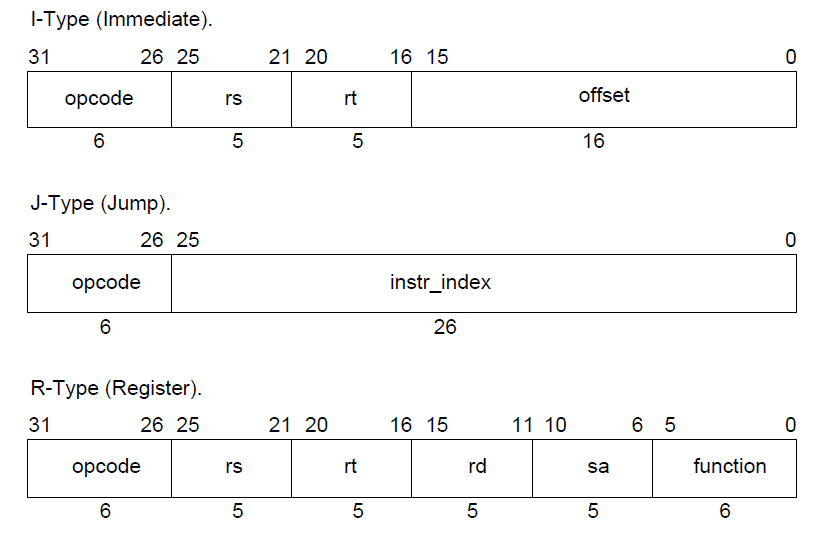
\includegraphics[width=\textwidth]{formats.png}
\end{center}
\caption{MIPS-I instruction formats}
\label{formats}
\end{figure}

In all J-TYPE and I-TYPE instructions
(except branch instructions comparing one register against zero),
the opcode field is used to specify instruction type. This class
of instructions is called `instructions encoded by opcode field'.
All possible values for opcode field under this class are shown
in figure \ref{encoding1}, along with valid mnemonics.\\

\begin{figure}[H]
\begin{center}
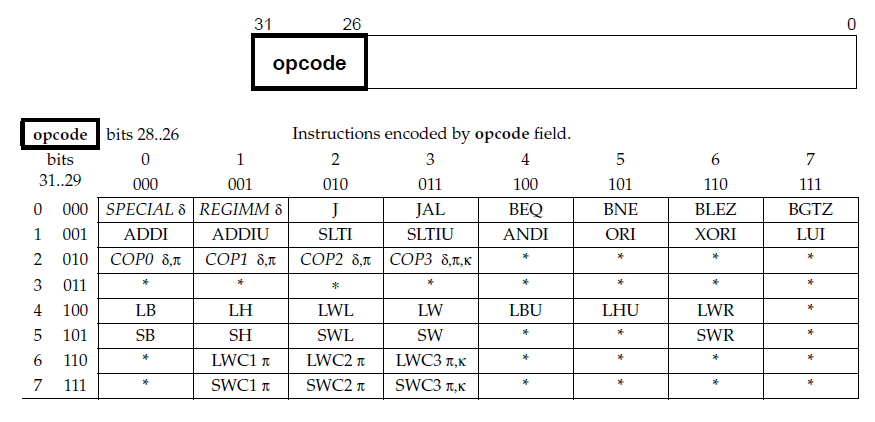
\includegraphics[width=\textwidth]{encoding1.png}
\end{center}
\caption{Instructions encoded by opcode field}
\label{encoding1}
\end{figure}

All R-TYPE instructions (including control instructions)
are encoded using funct field, where opcode field is constant.
For control instructions, the opcode field is equal to $COP0$ constant,
while opcode field of remaining instruction is equal to $SPECIAL$ constant.
R-TYPE instructions with opcode equal to $SPECIAL$ constant form
another third class, called `instructions encoded by function field
when opcode field = $SPECIAL$'. Figure \ref{encoding2} shows
members of this class.\\

\begin{figure}[H]
\begin{center}
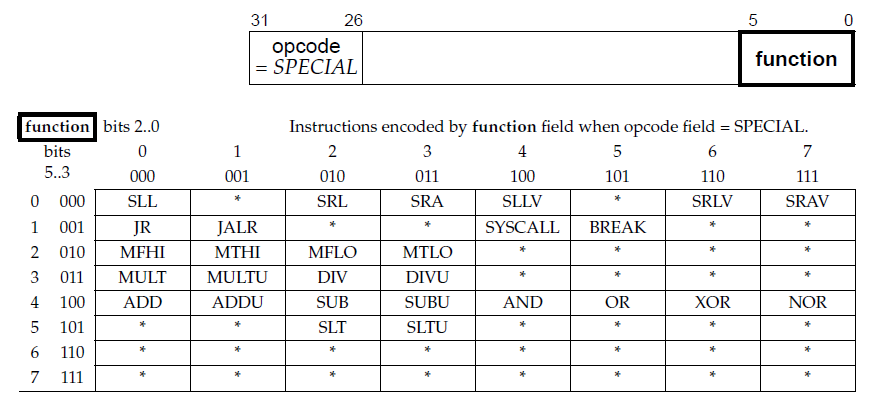
\includegraphics[width=\textwidth]{encoding2.png}
\end{center}
\caption{Instructions encoded by function field when opcode field = $SPECIAL$}
\label{encoding2}
\end{figure}

Finally, branch instructions comparing one register against zero are
encoded using rt field, while opcode field hold a constant value
equal to $REGIMM$ constant (register-immediate).
This class, shown in figure \ref{encoding3}, is called `instructions
encoded by the rt field when opcode field = $REGIMM$'.\\

\begin{figure}[H]
\begin{center}
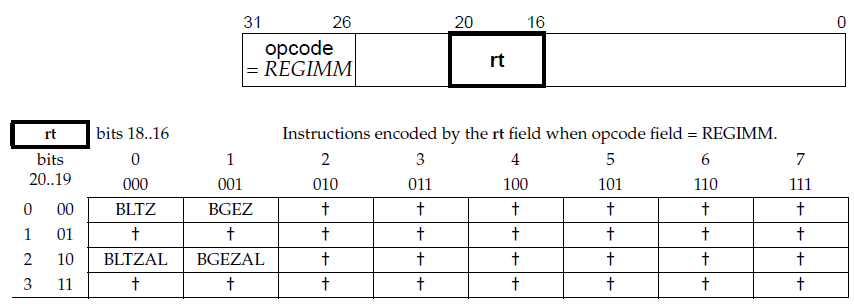
\includegraphics[width=\textwidth]{encoding3.png}
\end{center}
\caption{Instructions encoded by rt field when opcode = $REGIMM$}
\label{encoding3}
\end{figure}

\subsubsection{Addressing Modes}

Figure \ref{addrmodes} summarizes all possible addressing modes
along with instructions that support them:

\begin{figure}[H]
\begin{center}
\resizebox{0.9\textwidth}{!} {
\begin{tabular}{|c|c|}

\hline \textbf{Addressing Mode} &
       \textbf{Corresponding Instructions} \\

\hline Register, [Base Register]+Immediate Offset &
       Load/Store Instructions \\

\hline Register, Register, Immediate &
       ALU Instructions with Immediate Operand \\

\hline \multirow{2}{*}{Register, Register, Register} &
       ALU Instructions with Three Operands \\
\cline{2-2} & SLLV, SRLV, and SRA \\

\hline Register, Register, Shift Amount &
       SLL, SRL, and SRA \\

\hline Register, Register &
       MULT, MULTU, DIV, and DIVU \\

\hline Register &
       MFHI, MTHI, MFLO, and MTLO \\

\hline Absolute Address Within 256MB Segment &
       Jump Instructions Jumping Within 256MB Region \\

\hline Register Absolute &
       Jump Instructions to Absolute Address \\

\hline Register, Register, PC-Relative Immediate &
       Branch Instructions Comparing 2 Registers \\

\hline Register, PC-Relative Immediate &
       Branch Instructions Comparing Against Zero \\

\hline Immediate Code &
       Exception Instructions \\

\hline Register, Control Register &
       MFC0 and MTC0 \\

\hline Implicit &
       TLBR, TLBWI, and RFE \\

\hline

\end{tabular}
}
\end{center}
\caption{All possible addressing modes}
\label{addrmodes}
\end{figure}

We note that every instruction has no more than one single addressing
mode, thus MIPS doesn't need an addressing mode field in instruction
word.

\subsubsection{Programmer-Visible Pipeline Effects}

Several effects related to the behaviour of the pipeline should be stated
clearly so the programmer can be aware of the exact performance parameters
of the running program:

\begin{itemize}

\item \textbf{Delayed branching}: Since the effective address is not available
      immediately after fetching a jump/branch instruction, a delay
      slot should be inserted after the jump/branch instruction. The
      delay instruction is always fetched and executed after the
      jump/branch instruction. The effective address becomes ready
      after fetching the delay instruction and next instruction
      would be the instruction at the new PC.

\item \textbf{Load data not available}: If a memory load instruction is
      followed by an ALU instruction that requires the data
      acquired by the load instruction (addresses the same
      register), a data hazard will occur since ALU must wait
      until MEM unit is done fetching data from memory. This
      shall delay the execution of the ALU instruction by
      one delay slot (stalls the pipeline for one slot).

\item \textbf{Consequent control instructions}: A control instruction
      may stall if there is another control instruction
      in the pipeline, to prevent data hazards and simultaneous
      access to TLB and stuff.

\item \textbf{Branch instruction operands not ready}:
      If a branch instruction depends on result of the previous
      instruction (or second previous instruction), the pipeline
      will stall until data is ready.

\item \textbf{Multiply/divide instructions}: These four special
      instructions take more than one CPU clock cycle to complete,
      therefore they might stall the pipeline.

\item \textbf{Cache misses}:
      The pipeline shall stall if the instruction to
      be fetched or data specified by load instruction is not in cache.
      Furthermore, store instructions would always stall the pipeline
      since the cache system is write-through. This means that an
      instruction will take more than one CPU clock cycle if a cache
      miss happens.

\item \textbf{Unaligned memory access}:
      This class of instructions shall take
      more than one CPU clock cycles because atomic access to unaligned
      word is not possible.

\end{itemize}

Other than the cases specified above, the pipeline will have no
hazards/stalls and every instruction will take no more than one clock cycle
delay.

\subsection{Registers}

A register is a small amount of memory that can be accessible
faster than memory/cache. Processor provides direct register
access through `register' addressing mode.\\

MIPS architecture defines number of registers to be used
as general-purpose registers by the running software. MIPS
architecture also defines two special-purpose registers called
LO and HI registers.\\

In addition to registers defined by MIPS standard, our processor
contains special registers that control the behaviour of the processor,
called `control registers'. Surprisingly, control registers are
accessible through control instructions.\\

\subsubsection{General-Purpose Registers}

Strictly speaking, MIPS architecture doesn't make any assumptions
about the use of the 32 general-purpose registers. It's up to the
programmer to use the register the way she likes, and the hardware
will just perform the operations on those registers as specified
by the programmer. However, there are two exceptions to this:

\begin{enumerate}

\item Register 0 is always zero, no matter what value the programmer
      writes to it.

\item Register 31 is used as a link register (register containing
      return address from subroutine). Some instructions implicitly
      address this register.

\end{enumerate}

Although MIPS architecture doesn't make any assumptions on the use
of general-purpose registers (except for register 0 and 31), people
used to use those registers according to conventions listed in
figure \ref{regs}. The figure shows conventional names and uses
associated with the registers. Available assemblers and compilers
for MIPS architecture are expected to follow the same conventions.

\begin{figure}[H]
\begin{center}
\resizebox{0.9\textwidth}{!} {
\begin{tabular}{|c|c|c|}

\hline \textbf{Reg\#} & \textbf{Name}  & \textbf{Description} \\

\hline 0     & zero  & Always zero \\

\hline 1     & at    & Used by assembler ($at = assembler\ temporary$) \\

\hline 2-3   & v0-v1 & Value returned by subroutine \\

\hline 4-7   & a0-a3 & Subroutine parameters ($a\# = argument\#$) \\

\hline 8-15  & t0-t7 & \multirow{2}{*}{
                       Used by subroutines without saving
                       ($t\# = temporary\#$)} \\
\cline{1-2} 24-25 & t8-t9 & \\

\hline 16-23 & s0-s7 & Must be saved before use
                       ($s\# = subroutine\_var\#$) \\

\hline 26-27 & k0-k1 & Used by exception handler \\

\hline 28    & gp    & Global pointer \\

\hline 29    & sp    & Stack pointer \\

\hline 30    & s8/fp & 9th register variable/frame pointer \\

\hline 31    & ra    & Return address \\

\hline

\end{tabular}
}

\end{center}
\caption{Conventional names/uses of MIPS registers}
\label{regs}
\end{figure}

\subsubsection{LO and HI Registers}

Along with the 32 registers defined above, two special registers
are defined by the MIPS architecture to store results of MULT, MULTU,
DIV, and DIVU instructions. Since these four instructions produce
64-bit results, they need two destination registers. Since MIPS
architecture doesn't define more than one destination register
for an instruction (for hardware considerations), the result
should first stored in an intermediate 64-bit register (or two
parallel 32-bit registers) then moved to the GPRs in two steps.\\

The intermediate registers are called LO and HI registers. Each
one of them is 32-bit wide, so you can see them as one 64-bit
register which is can be accessed in halfs. LO
and HI can be read using MFLO and MFHI instructions, each of which
copies the value of LO or HI register into a general-purpose register.
The HI and LO registers can also altered by MTLO and MTHI instructions.

\subsubsection{Control Registers}

Now we turn our attention to the last class of registers, registers
that control the behaviour of the processor. These registers are
not defined by MIPS architecture itself, yet a processor needs
to have a set of registers to store control switches. These
registers are analogous to CR0, CR2, CR3, and EFLAGS registers of
x86 architecture.\\

Control registers are accessible only through MFC0 and MTC0 instructions,
which transfer values between GPRs and control registers. Every control
register is addressed by a special index. Figure \ref{ctrlregs} shows
all the control registers of our processor and their uses. \\

\begin{figure}[H]
\begin{center}
\resizebox{0.9\textwidth}{!} {
\begin{tabular}{|c|c|c|}

\hline \textbf{Reg Indx} & \textbf{Name}  & \textbf{Description} \\

\hline 0     & Index    & Stores index of TLB entry to be read/written \\

\hline 2     & EntryLo  & The lowest half of TLB entry to be read/written \\

\hline 9     & BadVaddr & Stores the memory address that caused TLB miss \\

\hline 10    & EntryHi  & The highest half of TLB entry to be read/written \\

\hline 12    & SR       & Status register \\

\hline 13    & Cause    & Exception type \\

\hline 14    & EPC      & Address of the instruction that caused an exception\\

\hline

\end{tabular}
}

\end{center}
\caption{Control registers}
\label{ctrlregs}
\end{figure}

Every control register has a specific format with a special function
for every field. Next we show the format of every control register
with a detailed description for the fields and how they can be used.\\

\begin{itemize}

\item \textbf{\underline{Index Register:}}\\

\begin{figure}[H]
\begin{center}
\begin{tabular}{|c|c|c|c|c|}

\hline \multicolumn{5}{|c|}{Index Register (0)} \\

\hline \textbf{Field bit(s):} & 31 & 30..14 & 13..8 & 7..0 \\

\hline \textbf{Field name:}   & 0  & x      & Index & x    \\

\hline

\end{tabular}

\end{center}
\caption{Format of Index register}
\label{index_reg}
\end{figure}

Detailed description for fields in figure \ref{index_reg}:

\begin{itemize}

\item \textbf{Index}: Before the operating system reads
      or modifies a TLB entry, it shall first write the
      index for the target TLB entry in this field using
      MTC0 instruction. After then, the OS issues a TLB
      read or TLB write using TLBR or TLBWI instruction.
      Index takes a value from 0 to 63, which implies
      that our TLB has 64 entries.

\end{itemize}

\item \textbf{\underline{EntryLo Register:}}\\

\begin{figure}[H]
\begin{center}
\begin{tabular}{|c|c|c|c|c|}

\hline \multicolumn{5}{|c|}{EntryLo Register (2)} \\

\hline \textbf{Field bit(s):} & 31..12 & 11..10 & 9 & 8..0 \\

\hline \textbf{Field name:}   & PFN    & 0      & V & 0    \\

\hline

\end{tabular}

\end{center}
\caption{Format of EntryLo register}
\label{entrylo_reg}
\end{figure}

Detailed description for fields in figure \ref{entrylo_reg}:

\begin{itemize}

\item \textbf{V}: This field matches the valid bit (V) of the
                  TLB entry to be read or written by the OS.
                  Before the OS writes a TLB entry, it writes
                  the valid bit of the entry in this field. When
                  TLBWI instruction is issued, the V field of
                  EntryLo register is copied into the V field
                  of TLB entry addressed by Index register. On
                  the other hand, when a TLBR instruction is
                  executed, the V field of TLB entry addressed
                  by Index register is copied into V field of
                  EntryLo register; a read for EntryLo.V field
                  (using MFC0 instruction) reveals what
                  the value of the V field of the addressed
                  TLB entry was when TLBR was issued.

\item \textbf{PFN}: This field matches the physical frame number
                    (PFN) field of the
                    TLB entry to be read or written by the OS.
                    Before the OS writes a TLB entry, it writes
                    the PFN of the entry in this field. When
                    TLBWI instruction is issued, the PFN field of
                    EntryLo register is copied into the PFN field
                    of TLB entry addressed by Index register. On
                    the other hand, when a TLBR instruction is
                    executed, the PFN field of TLB entry addressed
                    by Index register is copied into PFN field of
                    EntryLo register; a read for EntryLo.PFN field
                    (using MFC0 instruction) reveals what
                    the value of the PFN field of the addressed
                    TLB entry was when TLBR was issued.

\end{itemize}

\item \textbf{\underline{BadVaddr Register:}}\\

\begin{figure}[H]
\begin{center}
\begin{tabular}{|c|c|}

\hline \multicolumn{2}{|c|}{BadVaddr Register (9)} \\

\hline \textbf{Field bit(s):} & 31..0    \\

\hline \textbf{Field name:}   & BadVaddr \\

\hline

\end{tabular}

\end{center}
\caption{Format of BadVaddr register}
\label{badvaddr_reg}
\end{figure}

Detailed description for fields in figure \ref{badvaddr_reg}:

\begin{itemize}

\item \textbf{BadVaddr}: When a TLB miss happens, the memory
      address that causes the TLB miss is copied in this
      field. There are two cases here:
      \begin{enumerate}
      \item If a TLB miss happens while fetching an instruction
            from memory, the address of the instruction is
            copied into BadVaddr field before the exception
            handler is called.
      \item If the instruction is fetched successfully, but it
            happens that the instruction is a load/store instruction,
            and a TLB miss happens during fetching/writing data
            from/to memory, the effective address of the data element
            addressed by this instruction is placed in BadVaddr before
            the exception handler is called.
      \end{enumerate}

\end{itemize}

\item \textbf{\underline{EntryHi Register:}}\\

\begin{figure}[H]
\begin{center}
\begin{tabular}{|c|c|c|}

\hline \multicolumn{3}{|c|}{EntryHi Register (10)} \\

\hline \textbf{Field bit(s):} & 31..12 & 11..0 \\

\hline \textbf{Field name:}   & VPN    & 0     \\

\hline

\end{tabular}

\end{center}
\caption{Format of EntryHi register}
\label{entryhi_reg}
\end{figure}

Detailed description for fields in figure \ref{entryhi_reg}:

\begin{itemize}

\item \textbf{VPN}: This field matches the virtual page number
                    (VPN) of the
                    TLB entry to be read or written by the OS.
                    Before the OS writes a TLB entry, it writes
                    the VPN field of the entry in this field. When
                    TLBWI instruction is issued, the VPN field of
                    EntryHi register is copied into the VPN field
                    of TLB entry addressed by Index register. On
                    the other hand, when a TLBR instruction is
                    executed, the VPN field of TLB entry addressed
                    by Index register is copied into VPN field of
                    EntryHi register; a read for EntryHi.VPN field
                    (using MFC0 instruction) reveals what
                    the value of the VPN field of the addressed
                    TLB entry was when TLBR was issued.

\end{itemize}

\item \textbf{\underline{Status Register:}}\\

\begin{figure}[H]
\begin{center}
\begin{tabular}{|c|c|c|c|c|c|c|}

\hline \multicolumn{7}{|c|}{Status Register (12)} \\

\hline \textbf{Field bit(s):} & 31..5 & 4   & 3 & 2   & 1 & 0  \\

\hline \textbf{Field name:}   & 0     & IEo & 0 & IEp & 0 & IEc \\

\hline

\end{tabular}

\end{center}
\caption{Format of Status register}
\label{status_reg}
\end{figure}

Detailed description for fields in figure \ref{status_reg}:

\begin{itemize}

\item \textbf{IEc}: Interrupt enable/disable flag. When software
      writes 1 to this field, interrupts are enabled. When software
      writes to this field, interrupts are disabled and do not trigger
      any exception. This field is reset to 0 by hardware on two events:

      \begin{enumerate}
      \item CPU is reset.
      \item An exception has taken place.
      \end{enumerate}

      This field is also modified by RFE instruction which copies the
      value of IEp field into IEc field.\\

      It's important to note that when an exception happens and the
      value of IEc is reset to 0, the old value of IEc is not lost
      but rather is copied into IEp. Also, the old value of IEp
      is copied into IEo before IEc is copied into IEp. When exception
      handler returns, RFE instruction is executed and the value
      of IEp is copied back to IEc, and the value of IEo is copied
      back to IEp.\\

      Actually, the three fields (IEc, IEp, and IEo) behave like
      a 3-level stack for the value of the interrupt flag. The
      top of the stack (IEc) is the current state of the interrupt
      flag. When an exception happens, a 0 is pushed into stack,
      causing interrupts to be disabled and the values of the
      three entries are shifted by 1 (IEp copied into IEo and
      IEc copied into IEp).\\

      If a nested exception occurs again,
      the process repeats, thus IEo shall then hold the old value
      of the interrupt flag, IEp shall hold the value of the
      interrupt flag during handling the first exception, and IEc will be
      reset to 0.\\

      When the exception handler returns, RFE instruction
      will cause the stack to pop; IEp will be copied back to IEc
      and IEo will be copied back to IEp, thus IEc returns
      back to its original state before the exception has occured.\\

      This behaviour allows an exception to be nested into
      another exception without need to push status register
      into the software stack before the inner exception happens.

\item \textbf{IEp}: As discussed above, this field functions as backup
      for IEc field during exception handling. The three fields
      (IEc, IEp, IEo) can be seen as a 3-level stack to store the value
      of the interrupt flag across exceptions.\\

      When an exception happens, the value of this field is copied into
      IEo field and the value of IEc is copied into this field before
      IEc is reset to 0. When an RFE instruction is executed, the value
      of this field is copied back to IEc and the value of IEo is copied
      into this field. \\

\item \textbf{IEo}: As discussed above, this field functions as backup
      for IEp field during exception handling. The three fields
      (IEc, IEp, IEo) can be seen as a 3-level stack to store the value
      of the interrupt flag across exceptions.\\

      When an exception happens, the value of IEp is copied into this field
      before IEc is copied into IEp. When an RFE instruction is executed,
      the value of this field is copied back to IEp. \\

\end{itemize}

\item \textbf{\underline{Cause Register:}}\\

\begin{figure}[H]
\begin{center}
\begin{tabular}{|c|c|c|c|c|}

\hline \multicolumn{5}{|c|}{Cause Register (13)} \\

\hline \textbf{Field bit(s):} & 31 & 30..7 & 6..2    & 1..0 \\

\hline \textbf{Field name:}   & BD & 0     & ExcCode & 0    \\

\hline

\end{tabular}

\end{center}
\caption{Format of Cause register}
\label{cause_reg}
\end{figure}

Detailed description for fields in figure \ref{cause_reg}:

\begin{itemize}

\item \textbf{ExcCode}: When an exception occurs, the type
      of the exception is copied into this field before
      the exception handler is called. Currently, only
      the types of exceptions shown in figure \ref{exccode}
      are supported.

      \begin{figure}[H]
      \begin{center}
      \begin{tabular}{|c|c|}
      \hline \textbf{ExcCode Value} & \textbf{Description} \\
      \hline 0                      & Interrupt Exception \\
      \hline 1                      & TLB Miss Exception \\
      \hline
      \end{tabular}
      \end{center}
      \caption{ExcCode values with their meaning}
      \label{exccode}
      \end{figure}

\item \textbf{BD}: When an instruction causes exception (or
      gets interrutpted), this field is set to 1 if the
      instruction is a delay slot instruction, otherwise
      it is reset to 0; thus `BD' means branch detected.

\end{itemize}

\item \textbf{\underline{EPC Register:}}\\

\begin{figure}[H]
\begin{center}
\begin{tabular}{|c|c|}

\hline \multicolumn{2}{|c|}{EPC Register (14)} \\

\hline \textbf{Field bit(s):} & 31..0 \\

\hline \textbf{Field name:}   & EPC   \\

\hline

\end{tabular}

\end{center}
\caption{Format of EPC register}
\label{epc_reg}
\end{figure}

Detailed description for fields in figure \ref{epc_reg}:

\begin{itemize}

\item \textbf{EPC}: When an instruction that is currently
      executed by the processor causes an exception (like
      TLB miss) or gets interrupted (by en external I/O device),
      the address of the instruction is copied into EPC field,
      then exception handler is called.
      If the instruction is a delay slot instruction, the address
      of the previous jump/branch instruction is copied into
      EPC field instead of the address of the delay slot instruction.\\

      This behaviour prevents software to misbehave when the exception
      handler returns (as the branch instruction needs to be executed
      again or the processor will keep fetching instructions that follow
      the delay slot no matter the branch is taken or not). This
      special case causes BD field of Cause register to set as
      described above.\\

      It's also important to note
      that before exception handler is called, the CPU makes
      sure that the instruciton doesn't have any effect on
      the architectural state of the processor (i.e, any
      effect caused by the instruction is undone).

\end{itemize}

\end{itemize}

\subsection{Memory Management}
\label{ssec:memman}

Having discussed the instruction set and registers of our CPU, we now
turn our attention to how the CPU translates memory accesses. When
an instruction is fetched from memory, or when a load/store instruction
requests data from memory, the memory address is first translated
by means of translation look-aside buffer (TLB). The translated
address is then used to look-up data in the cache which might then
issue an access request to main memory if data is not found in cache.
Figure \ref{memaccess} summarizes the process.\\

\begin{figure}[H]
\begin{center}
\begin{tikzpicture}

\draw[black, thick]
    (0,0)  node[minimum width =50, rectangle,
                minimum height=50, draw](w) {CPU Core}
    (4,0.25) node[minimum width =50, rectangle,
                minimum height=25, draw](x) {TLB}
    (8,0)  node[minimum width =50, rectangle,
                minimum height=50, draw](y) {Cache}
    (13,0) node[minimum width =50, rectangle,
                minimum height=50, draw](z) {Memory}
    ;
\draw[->, black, transform canvas={yshift=10}]
    ([yshift=-25]w) -- node[above]{\scriptsize logical address} (x);
\draw[->, black, transform canvas={yshift=2.7}]
    ([yshift=25]x) -- node[above]{\scriptsize physical address} (y);
\draw[->, black, transform canvas={yshift=10}]
    (y) -- node[above]{\scriptsize only on a cache miss} (z);
\draw[->, black, transform canvas={yshift=-13}]
    (z) -- node[below]{\scriptsize data returned} (y);
\draw[->, black, transform canvas={yshift=-13}]
    (y) -- node[below]{\scriptsize data returned} (w);

\end{tikzpicture}
\end{center}
\caption{Memory access levels}
\label{memaccess}
\end{figure}

The figure presents two different types of addresses: logical address
and physical address. We define both terms as follows:

\begin{enumerate}

\item \textbf{Logical address}: the address of a memory location or
an instruction from the prespective of the running program. This simply
means that a program doesn't see memory as it is in reality. The
running program doesn't need to know the real address of the memory
item it is currently addressing, but the operating system must
provide the mapping between the logical address of a memory item
and its real location in memory. This mapping is used by translation
circuitry that translates logical address to the real location
before main memory is queried.

\item \textbf{Physical address}: this is the real location of
the memory item or the instruction that is being accessed. Physical
address is the address that is put on the bus when main memory
access is established by the processor. Also, as will be seen later,
data in cache is looked up by its physical address, not
logical address.

\end{enumerate}

The reason why there are two separate types of addresses and a translation
circuitry is to allow every process to have its own address space by
providing a distinct logical-to-physical address mapping for every
running process. The process of translating a logical address
to its corresponding physical address is called
\textbf{address translation}. \\

Figure \ref{translation} illustrates how we can
achieve process-level isolation using this technique.
Every process has its own set of memory items: blue items belong
to process 1, and red items belong to process 2. The OS needn't
allocate the items in physical address space in a specific order
(they are scattered over memory) since the running program
doesn't need to know the physical locations and doesn't need
to make any assumptions about them.\\

\begin{figure}[H]
\begin{center}
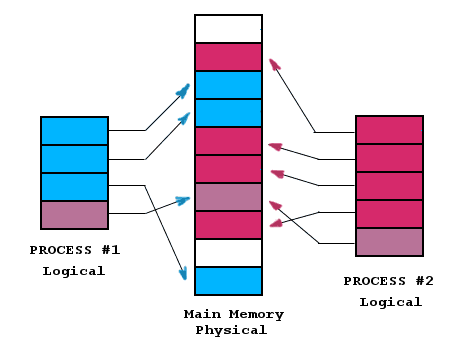
\includegraphics[width=0.6\textwidth]{translation.png}
\end{center}
\caption{Process logical address spaces and mappings to physical addresses}
\label{translation}
\end{figure}

The OS provides two separate mappings for both processes in the figure.
Each mapping provides enough information needed to translate
logical addresses of memory items belonging to the process to
physical addresses. Each process only sees its own items in the
logical address space, therefore a process can never access
memory items of other processes because there is no mapping for them.
By this mechanism, we have achieved the required isolation between
processes: every process can only access the items allocated to it.\\

The OS might allow some memory items to be shared between more
than one process. The purple item in the figure is seen in the
logical address space of both process 1 and process 2. This implies
that an item in main memory can have more than one logical address (for
several mappings). However, every memory item can have no more than
one physical address.\\

The process of allocating and organizing items in main memory is the
responsibility of the OS. Also, the OS is responsible for providing
the required mapping between logical and physical addresses. The OS
provides the CPU with the mapping of the process that is currently
being executed, and the CPU is responsible only for doing the translation
on every memory access. Later in this section we show how the OS
informs the CPU of the mapping. \\

It's important to note that some authors use terms like
`virtual address' and `program address' to refer to logical addresses.
We shall use the term `logical address' throughout the document to
prevent confusion with other terms and techniques, like `virtual memory',
which shouldn't be confused with `logical address space', or equivalently,
`logical memory'.\\

\subsubsection{MIPS Logical Address Space}

Since a logical address is 32 bits (as seen earlier), every process
shall has a logical address space of 4GB. This 4GB address space
is divided into four regions, each region is translated differently
as will be seen below. The four regions are:

\begin{enumerate}

\item \textbf{kuseg} 0x00000000 - 0x7FFFFFFF (2GB):
      any address in this region is translated by the translation
      circuitry to its corresponding physical address using the
      mapping provided by the OS. This area usually contains the
      text and data of the running process.

\item \textbf{kseg0} 0x80000000 - 0x9FFFFFFF (512MB):
      addresses in this region are not translated using the
      mapping provided by the OS, but rather they are translated
      by stripping off the most significant bit. Thus, this
      region simply maps to the physical region:
      0x00000000 - 0x1FFFFFFF. Operating system kernel can
      be simply put inside the lower 512MB zone of the
      main memory, and consequently it will appear inside kseg0.
      This implies that the kernel doesn't need to setup
      any mapping for itself, it is just mapped automatically
      to this region. This also implies that kernel memory
      area is shared among all processes.

\item \textbf{kseg1} 0xA0000000 - 0xBFFFFFFF (512MB):
      just like kseg0, addresses in this region also translate
      to the lower 512MB of physical address space. The only
      difference between kseg0 and kseg1 is that memory access
      of any address in kseg1 will skip the cache, so it is
      always uncached, while kseg0 is always cached. Access
      to memory-mapped I/O registers should always be done
      through this segment (to prevent caching). System
      designers must make sure that I/O registers have
      physical addresses in the low 512MB physical zone so that
      they can appear in kseg1.

\item \textbf{kseg2} 0xC0000000 - 0xFFFFFFFF (1GB):
      any address in this region is simply translated
      using the mapping provided by the operating system,
      this area is usually used to contain OS data structures
      which are maintained by the kernel.

\end{enumerate}

We conclude that addresses in kuseg and kseg2 are translated
the same way, using the mapping provided by the operating system,
while addresses in kseg0 and kseg1 are translated by mapping them
directly to the lower 512MB zone of physical memory. The only
difference between kseg0 and kseg1 is that the former is cached
while the later is uncached. The difference between kuseg and kseg2
is that kuseg is used to hold current process code and data,
while kseg2 is used to hold kernel objects.\\

Having a static mapping for kseg0 and kseg1 has several advantages:

\begin{enumerate}

\item Processor reset vector is put in kseg1. Consequently, system
      initialization code (i.e, firmware) can start execution
      before translation circuitry is initialized. Caching also
      might not be wanted during system initialization, thus
      kseg1 is a safe place to start the system from.

\item Kernel is shared among all processes and doesn't need a specific
      mapping. This means that kernel initialization code can be
      executed before the translation circuitry is initialized. This
      also implies that a system call from process code running in
      kuseg can be handled in kseg0 without need to switch logical address
      space (i.e, without providing translation circuitry with another
      mapping). Microkernels can also use this area to put the tiny
      code that does the logical address switching.

\end{enumerate}

When a process switch occurs, the OS must alter the translation
circuitry with the mapping of the new process. The kernel
can fix the mapping of kseg2 among all processes. Consequently, kernel
objects can also be shared by all processes, allowing system calls
to be handled without need to switching logical address space
or alter the mapping.

\subsubsection{Translation Look-aside Buffer (TLB)}

Now we show how the operating system provides the CPU with a certain
mapping for current process. Since there are 3GB of the address
space (kuseg and kseg2 regions, see above) that can be dynamically
mapped to physical memory, we need a data structure that describes
how to map every logical address inside the two regions (kuseg and
kseg2) into physical address. \\

One can think of an array of 4G elements, where the index of the array
is the logical address, and the contents of an array element is
the physical address that maps to the logical address associated
with that entry. Notice that the third quarter of such an
array would always be sparse, since kseg0 and kseg1 are not dynamically
mapped as shown before. \\

Since a physical address is 32 bits, we need an array of 4Gx4B which
is a 16GB data structure for every process. This is certainly
unfeasible and we would need to think for another solution.
Instead of mapping each logical address to a certain physical address,
we can map every block of logical address to a block of physical addresses.\\

Using this technique, we just need an array with n elements, where
n is number of blocks of the logical address space which is also
equal to number of block of the address space. We call this scheme
\textbf{`Paging'}, where a physical address is called a `frame'
and logical address block is called a `page'. \\

Given a page size of 4KB, the 4GB address space could be divided
into 1M pages, requiring an array of only 1M elements. The array
is called a `page table' and maps every page of the logical address
space to a frame in the physical memory. A page table entry
will simply contains the number of the frame it maps to, which
is a 20-bit word (because we've got a total number of 1M frames). \\

Extra information might need to be stored along with frame number,
like whether this page is mapped or not (a page can be unmapped
if doesn't map to any physical address) as well as OS-specific flags.
Hence we can extend the 20-bit entry to 32 bits: 12 bits for flags
and 20 bits for frame number (FN). Hence we need an array of 1M*4B
which is equal to 4MB page table for every process. This is much
smaller than 16GB. \\

To translate a logical address, we divide the address into two parts:
\begin{enumerate}
\item Page number: the highest 20 bits of the address
\item Offset inside the page: the lowest 12 bits of the address.
\end{enumerate}
Page number is then used to index the page table to get the
corresponding page table entry. The frame number is extracted
from the entry and concatenated with the 12-bit offset to form
the actual physical address that this logical address maps to.
Figure \ref{pagetable1} illustrates this translation process.

\begin{figure}[H]
\begin{center}
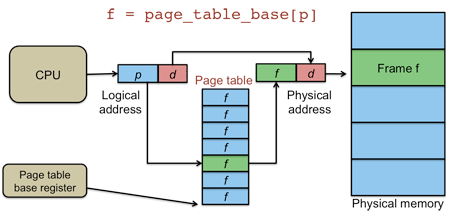
\includegraphics[width=0.6\textwidth]{pagetable1.png}
\end{center}
\caption{Address translation using page table}
\label{pagetable1}
\end{figure}

A page table of 4MB fo every process is still big, since when
number of processes increase, a big portion of main memory will
just be used to store page tables. Furthermore, a process
won't usually need to map the whole 4GB address space. It can leave
some pages unmapped, and only map pages where it needs to put
its code and data. Actually, the usual case is that most pages are
unmapped. And if virtual memory is not implemented, the total
number of mapped pages across all page tables (across all processes)
must be less than or equal to size of RAM (given that no frame
is mapped to by more than one page), and RAM is usually
much smaller than 4GB.\\

Since most entries in the page table are sparse (because most pages
in the logical address space are unmapped), the OS can make use
of this characteristic to make the size of the page table smaller.
Thus two-level page tables where introduced. The big 1M-entry page
table is divided into 1024 parts, with each part having 1024 entries.
Each part is called a second-level page table. These second-level
page tables could be scattered around memory. An 1024-entry table
could be used to store the addresses of these 1024 2nd-level tables.
Figure \ref{pagetable2} shows how translation works under this
two-level scheme.

\begin{figure}[H]
\begin{center}
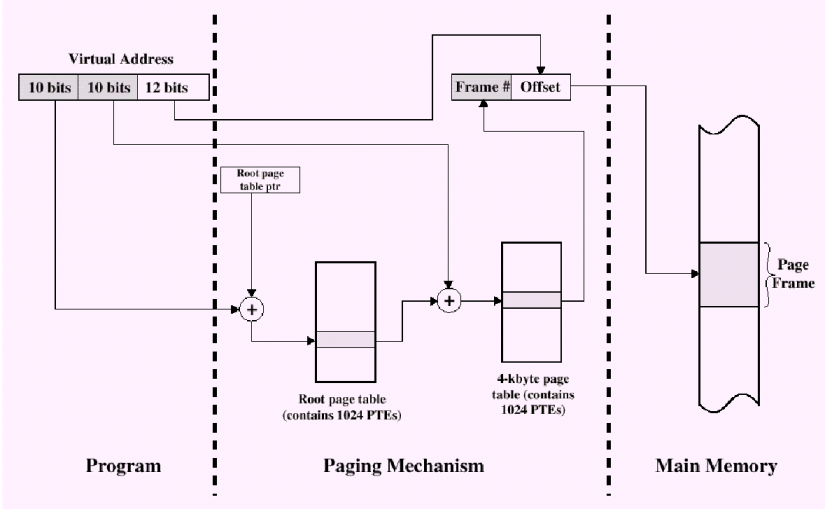
\includegraphics[width=0.75\textwidth]{pagetable2.png}
\end{center}
\caption{Address translation using two-level page table scheme}
\label{pagetable2}
\end{figure}

This way, if all the entries of a second-level page tables are
unmapped, the whole second-level page table could be unmapped,
setting a flag in the page directory that this page table
doesn't exist at all, and all pages in this region are unmapped.
Consequently, many second-level page tables wouldn't need to
exist at all, reducing the size of allocated memory for page
tables to a reasonable limit. However, if the process maps
all of its logical memory, page table increases to 4MB plus
the 4KB of the page directory. \\

This result implies that we cannot store the whole page table
in the processor, since we would need 4MB of memory inside
the CPU dedicated for page table. We would also need
to re-initialize the whole 4MB on every process switch, a process
that will take much time. That's why page tables are stored
in memory and with a multi-level scheme to redcue their sizes.\\

So, how the CPU makes use of these page tables to do translation?
The processor could simply be given the base physical address
of the page directory that controls the current process. When
a logical address is generated by core processor, the translation
circuitry looks up the page directory then the corresponding 2nd-level
page table to get frame number, as shown in the figure above.
On a process switch, the CPU is given the page directory of
next process.\\

This translation scheme requires two memory access for each translation,
which is too much since memory access takes much time, so we need
to cache page entries that are used frequently. Caching page
entries will effectively reduce average translation time.
This special-purpose cache is called \textbf{`translation
look-aside buffer'}, or simply TLB. When a logical address is generated
by core processor, TLB is queried for that logical address. If
the entry of this address is found inside TLB, the physical
address is returned immediately. If a TLB miss happens, the processor
shall access main memory to get page entry.\\

The type of TLB described above is called \textbf{`hardware-managed TLB'},
where TLB is totally isolated from the OS and is managed by
hardware. Another mechanism would be \textbf{`software-managed TLB'},
where TLB is controlled by the OS, and CPU doesn't need
to know any information about page table. In a software-managed TLB,
when a TLB miss happens, the CPU raises an exception, and it is
the responsibility of the exception handler to look-up page
tables and refill TLB with the missed entry.\\

Since our processor is designed for systems where resources
are very limited (like FPGA), we chose to use software-managed
TLB to simplify the implementation of the processor. On a process
switch, the OS just needs to clear TLB from entries related
to old process. After TLB is cleared, and when a logical address
is generated, a TLB miss happens and exception handler is called.
The OS queries page tables and refills TLB. Page tables are
totally managed by the OS; the processor doesn't need
to know anything about their structure and locations. \\

The TLB consists of 64 entries. Every entry is 64-bits wide
with the structure illustrated by figure \ref{tlb_entry}.

\begin{figure}[H]
\begin{center}
\begin{tabular}{|c|c|c|c|c|c|c|}

\hline \multicolumn{7}{|c|}{TLB Entry} \\

\hline \textbf{Field bit(s):} & 63..44 & 43..32 & 31..12 & 11..10 & 9 & 8..0 \\

\hline \textbf{Field name:}   & VPN    & 0      & PFN    & 0      & V & 0    \\

\hline

\end{tabular}

\end{center}
\caption{Format of TLB entry}
\label{tlb_entry}
\end{figure}

Fields are:

\begin{itemize}

\item \textbf{VPN}: the 20-bit logical page number to be translated.

\item \textbf{PFN}: the 20-bit physical frame number this VPN maps to.

\item \textbf{V}: valid bit. If this bit is set to 1, this is entry
      is valid and can be used for translation. If this bit is set to
      0, this entry is not valid and won't be used for translation.

\end{itemize}

The reader can notice the similarity between TLB entry and EntryLo/EntryHi
registers. The structure of the lower 32 bits of a TLB entry is identical
to EntryLo register, and the structure of the upper 32 bits is identical
to EntryHi register. EntryLo and EntryHi registers, along with Index
register, are used to read and write TLB entries. For reading a TLB
entry, the steps are:

\begin{enumerate}

\item The OS writes the index (0->63) of the TLB entry to be read into
      Index register using MTC0 instruction.

\item TLBR instruction is executed. The instruction causes the lower 32
      bits of the TLB entry indexed by Index register to be copied into
      EntryLo register, and the upper 32 bits of the TLB entry to be copied
      into EntryHi register.

\item The operating system reads EntryLo register using MFC0 instruction.
      Result is the lower 32 bits of the target TLB entry.

\item The operating system reads EntryHi register using MFC0 instruction.
      Result is the upper 32 bits of the target TLB entry.

\end{enumerate}

A similar sequence could be used for writing a TLB entry

\begin{enumerate}

\item The OS writes the index (0->63) of the TLB entry to be written into
      Index register using MTC0 instruction.

\item The operating system writes the lower 32 bits of the target TLB
      entry into EntryLo register using MTC0 instruction.

\item The operating system writes the upper 32 bits of the target TLB
      entry into EntryHi register using MTC0 instruction.

\item TLBWI instruction is executed. The instruction causes EntryLo register
      to be copied into the lower 32 bits of the TLB entry indexed by Index register,
      and EntryHi register to be copied into the upper 32 bits of the target
      TLB entry.

\end{enumerate}

Now since the operating system has full access to TLB, paging can be
implemented easily. Whenever a logical address is generated by
the processor, the following steps happen:

\begin{enumerate}

\item The CPU reads TLB entry which has an index that is equal to
      bits 12 to 17 (inclusive) of the logical address.

\item If V flag of the read entry is 0, the CPU copies the logical
      address into BadVaddr register, and TLB miss exception happens.
      In this case translation stops. If V flag is 1, continue to
      step 3.

\item The VPN of the read field is compared with the highest 20
      bits of the logical address. If both values are not equal,
      the logical address is copied into BadVaddr register and
      TLB miss exception happens. In this case translation stops.
      If both values are equal, continue to step 4.

\item The PFN of the read field is concatenated with the lower
      12 bits of the generated logical address, the result is
      the physical address that will be used to access memory.
      Translation is done and the CPU continues work normally
      without exception.

\end{enumerate}

Step 1 implies that our TLB is actually a \textbf{direct-mapped cache}
where the index is computed using bits 12 to 17 of the logical address,
and tag is VPN. Using this information, the OS can handle TLB miss exception
as follows:

\begin{enumerate}

\item The OS reads the value of BadVaddr register using MFC0 instruction.

\item The OS then queries page tables to know the mapping of the address
      in BadVaddr register. If there is no mapping, the operating system
      may decide to stop the program or send an error signal for instance.
      If there is mapping, the operating system reads the physical
      frame number that this logical address maps to.

\item The operating system calculates the index of the TLB entry which
      should be modified to solve the miss. The index is actually
      equal to bits 12 to 17 (inclusive) of the logical address as
      explained above.

\item Now the OS has the index, VPN, and the corresponding PFN. The OS
      simply writes the index to Index register, writes VPN to EntryHi
      register, and writes PFN to EntryLo register (and sets V flag
      of EntryLo register to 1).

\item The OS executes TLBWI instruction. EntryLo and EntryHi registers
      are then copied into the TLB entry.

\item Exception handler returns and the instruction that causes the miss
      is executed again, but this time it doesn't cause a TLB miss and
      execution continues normally.

\end{enumerate}

\subsubsection{Cache Memory}

After logical address is translated into physical address, physical
address is used to access RAM. However, because memory access
takes long time (i.e, has high penalty), a cache is put
between TLB and RAM to fasten memory access time.\\

Since the pipeline of our processor might be fetching an instruction
and handling memory access for a load/store instruction at the same time,
two separate caches are employed: an instruction cache and a data cache.
Both caches are direct-mapped caches. Every entry in the cache consists of
three fields:

\begin{itemize}

\item \textbf{Valid flag}: If 1, data and tag fields are valid. Otherwise
      the entry is invalid.

\item \textbf{Data field}: The 4-byte datum cached by this entry.

\item \textbf{Tag field}: A 20-bit field storing the higher 20 bits
      of the physical address associated with this entry.

\end{itemize}

Every cache has 1024 entries, resulting in two 4KB caches. The process
of looking up data in the cache is completely transparent from software.
Bits 2 to 11 (inclusive) of the physical address are used as index.
The tag of the entry at the calculated index is compared to the
higher 20 bits of the physical address. If valid bit is 1 and
comparison matches, data field of the entry is return to core processor.
If valid bit or 0 or comparison doesn't match, the CPU initiates
a memory cycle to bring data from RAM and updates the cache automatically.\\

Cache is write-through; any store instruction will cause data to
be written to both cache and RAM. A cache miss (or a store instruction)
causes the instruction to delay until data is brought from or written to
memory. However, cache hit can be handled without any delay; pipeline doesn't
stall and advance normally. Although caching is totally isolated from the
programmer, the programmer can use her knowledge of how cache works to
be able to write optimized programs that make full use of caching.

\subsection{Exception Handling}

In MIPS, an exception is a hardware event, trap, system call, or anything
that interrupts the normal flow of the program and needs special handling.
The same mechanism is used to handle all exceptions, which include:

\begin{itemize}

\item \textbf{Interrupts}: throughout this document, we will use
      the term `interrupts' to refer only to those generated by hardware
      devices. Interrupts are external events that need immediate
      interaction by the processor. Interrupts can be enabled/disabled
      by software (refer to Status Register). If enabled, when an
      interrupt signal arrives to the processor, exception happens
      and the normal flow of the program is interrupted. Interrupts
      may include, for example, keystrokes, mouse button events,
      and disk I/O events.

\item \textbf{System calls}: system calls are special calls that
      transfers the control to the operating system to execute
      some kernel-level subroutine then return back to user
      program and continue execution normally. System calls
      are handled by the processor as an exception trigger:
      when system call (or breakpoint) instruction is executed,
      an exception happens.

\item \textbf{Page faults}: page faults need to be reported to
      operating system whenever they happen to fully support
      paging. When a page fault happens, the running program is
      interrupted and exception handler is called. Exception
      handler shall handle the fault then return back to the
      running program.

\item \textbf{Program errors}: division erros, invalid opcodes,
      and invalid addresses are also forms of exceptions that
      cause the exception handler to be called. In this case
      the exception handler might, for example, call a specific
      signal handler in the faulty process or stop it completely.

\end{itemize}

Processor provide a mechanism to return from exception and resume
execution of the interrupted process. It's the responsibility
of the OS to store the context of the interrupted process
at beginning of exception handling, so that when the exception
handler returns back to the interrupted process, the process
continues its work normally as if nothing has happened.\\

It's the responsibility of the processor to inform software with
what kind of exception has actually happened, at which
instruction the exception has happened, and any extra parameters
needed. For example, if a program error has happened, the processor
shall inform software of which instruction has caused the error.
If a page fault happens, the processor should inform software
of which instruction caused the fault, and of the logical
address that couldn't be translated.\\

Up till now, we are talking about the concept of exceptions in
general, without projecting the concept on our architecture.
In the next lines we show how exceptions are designed in
our processor.

\subsubsection{Exception Cases}

Currently, these are all the events that cause our processor
to raise an exception:

\begin{itemize}

\item \textbf{Interrupt}: Only if IEc flag of SR register is 1,
      if IRQ signal arrives to the processor, the processor
      sets ExcCode field of Cause register to 0, copies the
      address of instruction that is currently being executed
      into EPC register, then calls exception handler. We note
      that there is only one IRQ signal that is fed to the processor.
      System designer should allow the IRQ signal to be shared by various
      I/O devices. Several techniques exist for sharing IRQ
      signals.

\item \textbf{TLB miss}: When logical address fails to be
      translated (as descibed earlier), the processor
      sets ExcCode field of Cause register to 1,
      copies the logical address into BadVaddr register,
      and copies the address of the instruction that
      has caused the TLB miss into EPC register. The processor
      then calls the exception handler.

\item \textbf{Reset signal}: Processor reset is also a form
      of exception, where the appropriate exception handler is
      called whenever this event happens. Reset doesn't cause
      the Cause register, EPC register, or any other registers
      to be modified. On RESET, software should re-initialize
      the processor and drives it to a known state.

\end{itemize}

It's important to note that when exception happens at some instruction,
the processor makes sure that all previous instruction has done execution
and their results has been commited successfuly before the exception
handler is called. The instruction at which the exception has happened
(the instruction whose address is copied to EPC) must not have
any effect on the architectural state of the processor, so that
when exception handler returns, the instruction can be re-executed
without problems. We will later introduce the concept of precise
exceptions.

\subsubsection{Exception Vectors}

Exception vector is the address where the exception handler is expected
to reside. When exception happens, the processor performs a far
jump to exception vector, starting from there the execution of
the exception handler. Actually, one distinct exception vector
could be assigned to every type of exception. In this case,
there is an exception handler for every type of exception.\\

Exception vectors could be static or dynamic. For static exception
vectors case, the vectors are predefined addresses that are hardwired
in the processor. Static vectors can never change. Examples
for architectures with static vectors include MIPS, 6502, and PIC
architectures.\\

Dynamic vectors are set up by software. They could be stored inside
one or more registers in the processor or could be stored in a table.
The table will contains vectors for all possible exception types.
Examples for architecture using dynamic vector mechanism include
x86 and Zilog Z80. In some architectures, like 68K and PDP-11,
the interrupting I/O device itself provides the processor
with the interrupt vector when an interrupt is handled.\\

Since MIPS processors use static hard-wired exception vectors, our
processor jumps to predefined addresses when exceptions happens.
Figure \ref{vectors} lists those predefined addresses and their
associated exceptions.

\begin{figure}[H]
\begin{center}
\begin{tabular}{|c|c|c|c|}

\hline \textbf{Logical Address} & \textbf{Region} &
       \textbf{Physical Address} & \textbf{Exception Types} \\

\hline 0xBFC00180  & kseg1 & 0x1FC00180 & All types of exception, except reset. \\

\hline 0xBFC00000  & kseg1 & 0x1FC00000 & Reset exceptions.\\

\hline

\end{tabular}
\end{center}
\caption{Excetion vectors for various exception types}
\label{vectors}
\end{figure}

We note that all exception handlers are located inside kseg1 memory
region. This is important for reset vector to be located in kseg1
region as it is the only safe region to start the system from
as explained before. Thus firmware location should be adjusted
in memory (by system designer) such that first instruction of
the firmware program matches reset vector.\\

The exception handler for other types of exception is also located
in the uncached kseg1 region. This might be necessary during
system initialization, but the OS later might want the exception
handler to be called through kseg0 (instead of kseg1) so that
it can be cached. A jump instruction could be inserted in
the exception handler at kseg1 for that purpose.

\subsubsection{Exception Protocol}

Except for reset exceptions, the processor does the following when
an exception happens:

\begin{enumerate}

\item Copy the address of the instruction that causes the
      exception into EPC register.

\item The 3-level stack inside SR register (explained before)
      is pushed and a 0 is inserted in IEc flag to disable
      interrupts.

\item Set the Cause register with appropriate ExcCode. If
      the exception is a TLB miss exception, the logical
      address is copied into BadVaddr register.

\item The processor transfers control to the exception handler.

\end{enumerate}

The exception handler should go through these steps:

\begin{enumerate}

\item Store the state (context) of the interrupted program. EPC
      should also be stored.

\item Load Cause register and examine ExcCode field to determine
      the type of exception and call the appropriate handler.

\item Process the exception. This can alter the values of
      registers and change the state of the processor, that's
      why the context of the interrupted process is stored in first
      step.

\item Restore the state of the interrupted program.

\item Return from exception: this can be done by loading the value
      of the EPC register (that is stored in step 1) into one of
      the general purpose registers, then using JR instruction to
      jump back to the instruction referred to by EPC. RFE instruction
      should be inserted into the delay slot of the JR instruction
      so that the stack in the SR register is popped just before
      returning to the interrupted program (to enable interrupts
      again). This is the safest method to return from exception.

\end{enumerate}

\subsubsection{Precise Exceptions}

We finally conclude our discussion with a note on the preciseness
of exceptions. Due to pipelining, multiple exceptions may
happen at the same time by various instructions in various
stages. Furthermore, an exception might happen in an instruction
where following instructions has already been executed and has
changed the architectural state of the processor.\\

To handle these pipeline issues, exceptions need to be `precise'.
An exception is called precise if the saved processor state
corresponds with the sequential model of the program execution,
although the underlying hardware excutes instructions in parallel
and out of order. In the case of precise exceptions, the OS
knows well that all instructions before the instruction referred
to by EPC have finished their execution successfully, and have
already committed their results. The OS also knows that
all instructions after EPC has never been executed and didn't
effect the processor state. These two points is what we mean
by saying that the saved processor state corresponds with
the sequential model of execution.\\

Since our prcoessor implements precise exceptions, it guarantees
the following:

\begin{itemize}

\item \textbf{Unambiguous proof of cause}: the values of EPC and
      Cause registers are exact and refer to the actual instruction
      that caused the exception and the actual type of exception.
      This wouldn't be the case on imprecise exceptions.

\item \textbf{Exceptions are seen in instruction sequence}:
       as described above, precise exceptions guarantees that
       all instructions before EPC has finished their execution
       successfully. If several exceptions at several stages happen
       at the same time, the processor choose the earlier instruction
       of them to be put in EPC. When an exception happens
       at some stage of the pipeline, exception handler is not
       called until all instructions in the following stages finish
       execution and commit their results.

\item \textbf{Subsequent instructions nullified}:
      all the stages before the stage that caused the exception
      are nullified and any change that happened by instructions
      in these stages is undone. This guarantees that all instructions
      after EPC can be restarted safely after exception handler returns.

\end{itemize}

\section{System Bus}

System bus is a set of signals that provide a communication mechanism
between the processor, memory interface, and various I/O devices. As
we have already explained, system bus consists of three sub-buses:

\begin{itemize}

\item \textbf{Address bus (32 lines)}: Contains the address
of the data word being read/written by CPU. Since the address bus
is 32 bits, the address space of our system has 4G addresses. The smallest
addressible unit is `byte'. Thus the whole address space is 4GB, with
every address referring to a distinct byte in memory.

\item \textbf{Data bus (32 lines)}: A bi-directional bus where CPU puts
data word that is to be written to memory, or memory puts data word that
is to be read by the processor. Since a data bus is 32 bits, the word size
of our bus is 32 bits. Byte and half-word accesses are also supported.

\item \textbf{Control bus}: This consists of a number of control signals
that control the communication between the processor and I/O devices. Details
on this will be seen below.

\end{itemize}

Address bus is always driven by the processor. No other devices are allowed to
drive the bus (or contention may happen). Data bus is driven either by the
processor (if data is to be written to memory) or by other devices (if
data is to be read by the processor). Control bus signals are driven by
various devices. Control bus supports these signals:

\begin{itemize}

\item \textbf{CLK}: clock signal to synchronize all components together. Generated
by clock circuitry and fed into all components.

\item \textbf{MEME}: memory enable signal, driven by CPU. When MEME changes from
inactive level to active level, a memory access cycle starts.

\item \textbf{RW}: read/write signal, driven by CPU. When inactive, CPU wishes to
read something from memory. When active, CPU wishes to write.

\item \textbf{DTYPE}: specify whether the CPU wants to read/write a single byte,
a half-word, or a word.

\item \textbf{IRQ}: IRQ signal controlled by interrupt controller. It is fed
into the processor and changes to active level when interrupt happens. The CPU
senses the inactive-to-active edge to detect interrupt requests.

\item \textbf{IAK}: interrupt acknowledge signal, driven by CPU and fed into
the interrupt controller. It changes
to active level when CPU wants to acknowledge the interrupt signal.

\item \textbf{IRQ\#}: 8 IRQ lines controlled by various I/O devices are fed into
the interrupt controller. When a device is interested in interrupting the
processor for some reason, it activates its own IRQ line.

\item \textbf{IAK\#}: 8 IAK lines controlled by the interrupt controller and fed
into various I/O devices. They are used to acknowledge the interrupt requests
issued by devices.

\item \textbf{CS\#}: chip select lines fed into the I/O devices and driven by
bus decoder. Bus decoder keeps listening to address bus. According to the
address loaded on the address bus, a device is selected and its own CS signal
changes to active level.

\end{itemize}

Now the sequence of a read/write cycle should be clear. First, the CPU puts
the target address on the address bus, sets DTYPE and RW signals, then raises
MEME to initiate the cycle. Bus decoder responds to MEME event by decoding
the address and driving the corresponding CS signal to the active level.\\

Next, the device whose CS signal has been activated knows it should respond to
the request. If RW is inactive (read cycle), the device puts data on the data
bus. Otherwise, the device fetches data from data bus and processes it.\\

\section{Bus Decoder}

Bus decoder is a simple address decoder that selects an I/O device based on
the state of the address bus. The decoder takes most significant bits of the
address as input, and selects the I/O device based on the value of these bits.
Thus, you can imagine the address space as a sequence of address blocks, where
each block belongs to a specific I/O device.\\

It should be clear by now that all I/O registers are mapped in the same
address space where memory is mapped. Therefore all I/O registers are
`memory-mapped registers' and no isolated I/O address space is supported.\\

Figure \ref{memmap} shows the memory map of our system. The decoder shall activate
the CS of a given device if and only if the address lies in the address range
dedicated to that device.

\begin{figure}[H]
\begin{center}
\begin{tabular}{|c|c|c|c|}

\hline \textbf{Start Address} & \textbf{End Address} &
       \textbf{Size} & \textbf{Device} \\

\hline 0x00000000 & 0x00FFFFFF & 16MB & RAM \\
\hline 0x1E000000 & 0x1E003FFF & 16KB & VGA \\
\hline 0x1E800000 & 0x1E800FFF &  4KB & KBD (Keyboard Controller) \\
\hline 0x1E801000 & 0x1E801FFF &  4KB & PIT (Programmable Interval Timer) \\
\hline 0x1E802000 & 0x1E802FFF &  4KB & PIC (Programmable Interrupt
                                                              Controller) \\
\hline 0x1F000000 & 0x1FFFFFFF & 16MB & ROM \\

\hline

\end{tabular}
\end{center}
\caption{Memory map.}
\label{memmap}
\end{figure}

It is important to note that there is a separate CS signal for RAM and
another separate CS signal for ROM. However, there is only one memory
interface circuit for interfacing both RAM and ROM chips. The interface
takes both CS signals as input, and selects whether to work with the
RAM chip or ROM chip based on the level of the signals.

\section{Memory Interface}

RAM and ROM chips have pinouts and interfaces that are not compatible
with the bus. Therefore there must be a circuit that converts between
both interfaces. The chips might not support 4-byte accesses (as will
be seen in the implementation chapter). Furthermore, control signals
need to be translated to the controls of the chips.\\

The circuit takes the lower 24 bits of the address bus as input (this
builds up to 16MB). CS\_ROM and CS\_RAM signals select whether the
24-bit address corresponds to RAM or ROM. The interface is designed that
way because the available RAM and ROM chips are actually 16MB each (as
will be explained later in the implementation chapter).\\

From programmer's point of view, ROM is accessed the same way as RAM.
If the address specified in LW/SW instruction corresponds to the
address range of RAM, then RAM chip is activated. Otherwise, if it
corresponds to the address range of ROM, then ROM chips is activated,
and that's all. The implementation details of the circuit are hidden
and do not affect the external behaviour seen by the programmer.\\

It is also important to note that writes to ROM (using SW instruction) are
just ignored. Since the chips need time until data is ready on
the data bus (or data has been written), the CPU should give the
circuit enough time before it deactivates MEME signal.

\section{VGA Interface}

This component provides an interface between our system and any CRT/LCD
screen with a VGA connector. VGA appears in the address space at the
range 0x1E00000-0x1E03FFF (16KB). Internally, the chip contains four
memory blocks of 2Kx9. This means that every block has 2K data units,
and every unit is 9 bits wide.\\

It is important to note that all memory addresses mentioned in this section
are physical addresses, refer to section \ref{ssec:memman} for more information
on address translation in MIPS architecture.\\

A write to one of the addresses in the range 0x1E00000-0x1E03FFF selects
a data unit in one (and only one) of the four RAM blocks.
Any write should be peformed using SH (store half) instruction, and
address should be always aligned to 2-byte boundary (i.e, lower 1 bit
should always be zero) as specified by MIPS architecture for SH instruction.\\

When a halfword is written to VGA, only lower 9 bits are conisdered, and
upper 6 bits are simply ignored. Figure
\ref{vgamap} shows how the blocks are selected based on the value
of the least significant 14 bits of the address.

\begin{figure}[H]
\begin{center}
\begin{tabular}{|c|c|c|}

\hline \textbf{Lower 14 Bits} & \textbf{Selected Block} & \textbf{Function} \\

\hline 0xxxxxxxxxxx00 & Block 0 & Character Memory \\
\hline 0xxxxxxxxxxx10 & Block 1 & Attribute Memory \\
\hline 1xxxxxxxxxxx00 & Block 2 & Font Memory 1 \\
\hline 1xxxxxxxxxxx10 & Block 3 & Font Memory 2 \\

\hline

\end{tabular}
\end{center}
\caption{VGA decoding mechanism.}
\label{vgamap}
\end{figure}

As you see, bit 0 is always 0, since writes are always 2-byte (half-word)
writes. The memory block is selected based on the value of bit 1 and bit 13.
This means that it is based on whether the address lies in the first half
or the second half of VGA address range, and whether the address (ignoring
bit 0) is odd or even. \\

So, to summarize the table, we can say that if the address lies in the
lower half of the VGA address range, then the address corresponds to
block 0 or 1 (character and attribute memories). If the address, ignoring
bit 0, is even, then select block 0. Otherwise (address is odd), select
block 1. \\

On the other hand, if the address lies in the upper half of the address range,
then the address corresponds to block 2 or 3 (font memories). If the address,
ignoring bit 0, is even, then select block 2. Otherwise (address is odd),
select block 3. \\

Now we know how a memory block is selected, the remaining part is to explain
how a data unit (inside the selected memory block) is addressed. You can
simply deduce that the remaining bits of the 14-bit address (the xxxxxxxxxxx)
are used directly as an index for the memory block. Thus, 00000000000 will
address the first data unit, where 00000000001 will address the second,
and so on. \\

If you look closely, you will find that the number of `x' bits is 11,
which means that we can address up to 2048 ($2^{11}$) for each memory
block. Every write is a 16-bit (half-word) write (with upper 6 bits
ignored), thus we are dealing with 2Kx9 units.\\

The reader can notice the similarity between our design and the design
of VGA programmer's interface of the IBM personal computer (the 0xB8000 text
buffer). The basic difference is that our memory blocks are 9 bits wide
(not 8), and that's the reason why writes are 16-bit writes, not 8-bit.

\subsection{Character Memory}

Our VGA module basically supports a 80x25 text mode. This means that screen
is divided into 80 columns and 25 rows (2000 cells), with every cell
containing an ASCII character. To draw text on screen, the operating system
just needs to specify the contents of the 2000 cells.\\

Character memory (memory bank 0) consists of 2048 9-bit cells (from 0
to 2047). Ignoring last 48 cells, cells from 0 to 1999 are used to describe
text on screen, with every cell corresponding to a character on screen.\\

To set the contents of character in row x (0-24), column y (0-79), you
need to use the formula: $indx=x*80+y$, then you can then refer to table
\ref{vgamap} which shows how to access the banks themselves.\\

For instance, to access row 2, column 1:

\begin{enumerate}

\item Calculate indx: $indx=2*80+1=161$.
\item We know we want to access bank 0, thus lowest 14 bits of the address
      will be 0xxxxxxxxxxx00 where bit 0 is zero as usual, bit 1 and 13 are 00,
      (to indicate bank 0), and xxxxxxxxxxx is the index.
\item Substitute xxxxxxxxxxx with 161, so it becomes 00010100001. Therefore,
      the lowest 14 bits are: 00001010000100 (0x0284).
\item The full 32-bit address can be easily deduced by ORing the lowest 14 bits
      with 0x1E000000, thus the full address is 0x1E000284.

\end{enumerate}

A write to 0x1E000284 will set the contents of cell 161 (which corresponds to
row 2, column 1). If you write 'B' (0x42 in ASCII) to address 0x1E000284, you
will see B shown on screen at third row (row 2) and second column (column 1).
That way you can write any kind of ASCII text you want on screen. Note that
bit 8 (highest bit) of a cell is always ignored, so only 256 ANSI symbols
are supported.

\subsection{Attribute Memory}

Bank 1 is used exactly the same way as bank 0, except that it describes
the colors, instead of the text itself. As we explained above, the screen
is divided into 2000 cells, organized in 25 rows and 80 columns. Every
cell has a corresponding 9-bit data cell in memory bank 0 containing ASCII
character that is drawn on the cell. Also, every cell has another
corresponding 9-bit data cell in memory bank 0 describing its color.\\

The format of the 9 bits is described as following:

\begin{itemize}

\item bits 0..3: color code of the ASCII character drawn in the cell
                 (foreground).
\item bits 4..7: color code of the background of the cell.
\item bit 8: you better set it to zero.

\end{itemize}

As it is clear, there are only 16 colors (coded by numbers from 0 to 15).
Color code are described in table \ref{colormap}.

\begin{figure}[H]
\begin{center}
\begin{tabular}{|c|c|c|c|c|c|c|c|}

\hline \textbf{Code} & \textbf{Color} &
       \textbf{Code} & \textbf{Color} &
       \textbf{Code} & \textbf{Color} &
       \textbf{Code} & \textbf{Color} \\


\hline 0 & \cellcolor{black}\color{white} Black        &
       4 & \cellcolor{red}\color{white}   Red          &
       8 & \cellcolor{darkgray}\color{white} Dark Gray    &
       C & \cellcolor{red!60}\color{white} Light Red    \\
\hline 1 & \cellcolor{blue}\color{white} Blue         &
       5 & \cellcolor{violet}\color{white} Violet       &
       9 & \cellcolor{blue!60}\color{white} Light Blue   &
       D & \cellcolor{violet!60}\color{white} Light Violet \\
\hline 2 & \cellcolor{green}\color{white} Green        &
       6 & \cellcolor{brown}\color{white} Brown        &
       A & \cellcolor{green!60}\color{black} Light Green  &
       E & \cellcolor{yellow}\color{black} Yellow       \\
\hline 3 & \cellcolor{cyan}\color{white} Cyan         &
       7 & \cellcolor{gray}\color{white} Gray         &
       B & \cellcolor{cyan!60}\color{black} Light Cyan   &
       F & \cellcolor{white}\color{black} White        \\

\hline

\end{tabular}
\end{center}
\caption{VGA color codes.}
\label{colormap}
\end{figure}

To set the color of the cell at row 2, column 1, we follow the same procedure
we followed when we set the text of the same cell in previous section:

\begin{enumerate}

\item Calculate indx: $indx=2*80+1=161$.
\item We know we want to access bank 1, thus lowest 14 bits of the address
      will be 0xxxxxxxxxxx10 where bit 0 is zero as usual, bit 1 and 13 are 01,
      (to indicate bank 1), and xxxxxxxxxxx is the index.
\item Substitute xxxxxxxxxxx with 161, so it becomes 00010100001. Therefore,
      the lowest 14 bits are: 00001010000110 (0x0286).
\item The full 32-bit address can be easily deduced by ORing the lowest 14 bits
      with 0x1E000000, thus the full address is 0x1E000286.

\end{enumerate}

So, to set the text of that cell, we write ASCII code (using SH instruction) to
0x1E000284. To set the color, we write the attribute to 0x1E00286. As we mentioned
before, bits 0..3 indicate the foreground color, where bits 4..7 indicate background.
For a white foreground (color code F) and blue background (color code 1), we
simply write 0x001F.\\

We conlude our discussion of character and attribute memory with a small
example to explain how to print something on screen. In this example,
we shall print `Hello World!' at row 0 of screen, with blue background
and white foreground. `H' will be written at column 0, `e' at column 1,
`l' at column 2, and so on.\\

We first type the text in character memory. Here we have 12 ASCII characters,
which will be written into cells from 0 to 11 of character memory. In table
\ref{hw1}, we  calculate the address of every cell of the 12 cells, and we
show the exact value that will be written in that cell using SH
(store halfword) instruction.\\

\begin{figure}[H]
\begin{center}
\begin{tabular}{|c|c|c|c|c|}

\hline \textbf{Row} & \textbf{Column} &
       \textbf{Memory Address} & \textbf{Text} & \textbf{ASCII code}  \\

\hline 0 & 0  & 0x1E000000 & H & 0x0048 \\
\hline 0 & 1  & 0x1E000004 & e & 0x0065 \\
\hline 0 & 2  & 0x1E000008 & l & 0x006C \\
\hline 0 & 3  & 0x1E00000C & l & 0x006C \\
\hline 0 & 4  & 0x1E000010 & o & 0x006F \\
\hline 0 & 5  & 0x1E000014 &   & 0x0020 \\
\hline 0 & 6  & 0x1E000018 & W & 0x0057 \\
\hline 0 & 7  & 0x1E00001C & o & 0x006F \\
\hline 0 & 8  & 0x1E000020 & r & 0x0072 \\
\hline 0 & 9  & 0x1E000024 & l & 0x006C \\
\hline 0 & 10 & 0x1E000028 & d & 0x0064 \\
\hline 0 & 11 & 0x1E00002C & ! & 0x0021 \\

\hline

\end{tabular}
\end{center}
\caption{Hello world example: text.}
\label{hw1}
\end{figure}

Next, we write the attributes of the 12 characters to attribute memory.
Since we want all characters to have white foreground (F) and blue
background (1), then color code is 0x1F. Table \ref{hw2} shows
the actual addresses that will be written.

\begin{figure}[H]
\begin{center}
\begin{tabular}{|c|c|c|c|c|}

\hline \textbf{Row} & \textbf{Column} &
       \textbf{Memory Address} & \textbf{Attributes} & \textbf{Color code}  \\

\hline 0 & 0  & 0x1E000002 & White/Blue & 0x001F \\
\hline 0 & 1  & 0x1E000006 & White/Blue & 0x001F \\
\hline 0 & 2  & 0x1E00000A & White/Blue & 0x001F \\
\hline 0 & 3  & 0x1E00000E & White/Blue & 0x001F \\
\hline 0 & 4  & 0x1E000012 & White/Blue & 0x001F \\
\hline 0 & 5  & 0x1E000016 & White/Blue & 0x001F \\
\hline 0 & 6  & 0x1E00001A & White/Blue & 0x001F \\
\hline 0 & 7  & 0x1E00001E & White/Blue & 0x001F \\
\hline 0 & 8  & 0x1E000022 & White/Blue & 0x001F \\
\hline 0 & 9  & 0x1E000026 & White/Blue & 0x001F \\
\hline 0 & 10 & 0x1E00002A & White/Blue & 0x001F \\
\hline 0 & 11 & 0x1E00002E & White/Blue & 0x001F \\

\hline

\end{tabular}
\end{center}
\caption{Hello world example: colors.}
\label{hw2}
\end{figure}

Addresses in tables \ref{hw1} and \ref{hw2} are calculated using the
procedure explained in the previous section and this section. By writing
the values to the addresses specified in the tables, `Hello World' is
printed on screen at row 0, as seen in figure \ref{hw3}.

\begin{figure}[H]
\begin{center}
\begin{tabular}{|c|c|c|c|c|c|c|c|c|c|c|c|c|c|c|c|}

\hline Row/Col & 0 & 1 & 2 & 3 & 4 & 5 & 6 & 7 & 8 & 9 & 10 & 11 & 12 & ... & 79 \\

\hline 0 & \cellcolor{blue}\color{white} H &
           \cellcolor{blue}\color{white} e &
           \cellcolor{blue}\color{white} l &
           \cellcolor{blue}\color{white} l &
           \cellcolor{blue}\color{white} o &
           \cellcolor{blue}\color{white}   &
           \cellcolor{blue}\color{white} W &
           \cellcolor{blue}\color{white} o &
           \cellcolor{blue}\color{white} r &
           \cellcolor{blue}\color{white} l &
           \cellcolor{blue}\color{white} d &
           \cellcolor{blue}\color{white} ! &
           \cellcolor{black} &
           \cellcolor{black} &
           \cellcolor{black} \\

\hline 1 & \multicolumn{15}{|c|}{\cellcolor{black}}\\
\hline 2 & \multicolumn{15}{|c|}{\cellcolor{black}}\\
\hline 3 & \multicolumn{15}{|c|}{\cellcolor{black}}\\
\hline 4 & \multicolumn{15}{|c|}{\cellcolor{black}}\\
\hline ... & \multicolumn{15}{|c|}{\cellcolor{black}}\\
\hline 24 & \multicolumn{15}{|c|}{\cellcolor{black}}\\

\hline

\end{tabular}
\end{center}
\caption{Hello world example: results on screen.}
\label{hw3}
\end{figure}

\subsection{Font Memory}

In previous sections we have shown how data stored in memory bank 0 (character
memory) and memory bank 1 (attribute memory) are used to draw text on screen.
The only remaining part is to describe the actual pixels inside every cell.\\

Every cell of the 2000 cells (on screen) consists of 16x9 pixels.
The width of the cell is 9 pixels and the height of the cell is 16 pixels.
Since the screen has 25 rows and 80 columns of cells, screen width is 80*9
which is equal to 720 pixels, and sreen height is 25*16 = 400.
This results in a resolution of 720x400, which is the default screen resolution
of many other systems, including IBM PC (during boot time).\\

Every ASCII character has a specific shape that is retrieved from bank 2 and
bank 3 to be drawn on screen. For example, if cell at row 0, column 0 contains
ASCII character `A', VGA hardware looks for the shape of `A' in bank 2 and bank 3.
A data cell in VGA memory is 9 bits wide. Since every cell of screen has 16 rows
and 9 columns of pixels, we can describe the shape of the cell using 16 9-bit
data cells, with one bit for every pixel.\\

This means that coloring inside data cell is monochrome; a pixel is either 0
or 1. If the color of the pixel is 0, VGA chooses to draw background color
described in the `attribute' memory as we explained before. On the other hand,
if pixel is 1, VGA chooses to draw the foreground color in that pixel.\\

For instance, consider the binary representation of letter `A' in figure
\ref{shape_a}. The representation consists of 16 rows, with every row having
9 bits (the size of a data cell). The whole 16x9 bits describe the whole
16x9 pixels of any cell having `A' in its character memory location,
as we explained before.

\begin{figure}[H]
\begin{center}
\color{black!50!blue!80}
\bfseries
\begin{BVerbatim}[showspaces=false,fontsize=\small]
row 0: 000000000 | 0x0000
row 1: 000000000 | 0x0000
row 2: 000010000 | 0x0010
row 3: 000111000 | 0x0038
row 4: 001101100 | 0x006C
row 5: 011000110 | 0x00C6
row 6: 011000110 | 0x00C6
row 7: 011111110 | 0x00FE
row 8: 011000110 | 0x00C6
row 9: 011000110 | 0x00C6
row A: 011000110 | 0x00C6
row B: 011000110 | 0x00C6
row C: 000000000 | 0x0000
row D: 000000000 | 0x0000
row E: 000000000 | 0x0000
row F: 000000000 | 0x0000
\end{BVerbatim}
\end{center}
\caption{Shape of letter `A' in font memory.}
\label{shape_a}
\end{figure}

So if cell 0 of bank 0 contains ASCII code of letter `A' (which is 0x0041),
and cell 0 of bank 1 contains color code of white foreground and blue
background (0x001F), VGA retrieves the shape of letter `A' (0x0041 in ASCII)
from bank 2 and bank 3. The retrieved data are the 16 9-bit words shown
in figure \ref{shape_a}.\\

Bits with value `0' describe pixels that will have the background color. Bits
with value `1' describe pixels that will have foreground color. The final
result is a matrix of 16x9 pixels drawn on screen, with letter `A' drawn
in white, over a blue background.\\

Bank 2 and 3 are called `font memory', since they are used to describe
the shapes of characters drawn on screen. Every ASCII character in the
ASCII character space is described using 16 9-bit words stored in bank 2
and bank 3. Since we have 256 possible characters (remember, bit 8 of
bank 0 is always ignored, so we only have 8 bits, from 0 to 7, to describe
a character), then we need $256*16 = 4096$ words, i.e, we need two banks.\\

The odd rows of a given ASCII character (row 1, 3, 5, ...) are stored in bank
3, while even rows are stored in bank 2. First 8 words of bank 2 describe
ASCII code 0, second 8 rows describe ASCII code 1, and so on... The same
structure is used in bank 3. The OS loads font data on booting, then starts
filling screen with ASCII characters by filling in bank 0 and 1.\\

\subsection{Special Registers}

As we mentioned before, VGA memory is mapped into 0x1E00000-0x1E03FFF.
We described how to access any location in the four memory banks which
all appear in this address region. However, there are several locations
inside this memory region that are reserved for special purposes. These
location are called `special registers'.\\

Special registers are written using SH instruction, the same way writes
to memory banks are performed. The only difference is that writes to
sepcial register locations are handled using special circuits. Table
\ref{vgaregs} shows all special registers and their locations.

\begin{figure}[H]
\begin{center}
\begin{tabular}{|c|c|c|c|c|}

\hline \textbf{Memory Address} & \textbf{Register Name} & \textbf{Function}  \\

\hline 0x1E001FFA & ROW\_BASE\_REG & Screen scroll location \\
\hline 0x1E001FFC & CURSOR\_ROW\_REG & Cursor row location \\
\hline 0x1E001FFE & CURSOR\_COL\_REG & Cursor column location \\
\hline

\end{tabular}
\end{center}
\caption{VGA special registers.}
\label{vgaregs}
\end{figure}

It is important to note that all these registers are 8 bits wide, so
bits 8-15 of the written half-word is always ignored. Now we shall
summarize the purpose of each register in the following points:

\begin{itemize}

\item \textbf{ROW\_BASE\_REG}:
Used to scroll up/down the screen. If this register is 0, screen is not
scrolled, and everything is displayed normally as expected. Otherwise,
this register shall contain the index of the row that will be displayed
on the top of the screen. For example, if this register contains 10, then
first row (the row on the top of screen) is row 10, next row is 11, and so on,
until we reach row 24. Next rows will be 0, 1, up to 9. This helps when the
OS needs to scroll up the screen by one row. The OS doesn't need to redraw
the whole buffer; instead it can just increase this register by 1, and clear
last row (the row at the bottom of the screen). Valid values for this
register are 0 to 24.

\item \textbf{CURSOR\_ROW\_REG}:
This specifies the row number where the blinking cursor appears. Valid
values are 0 to 24. Any other value will cause the cursor to be hidden.

\item \textbf{CURSOR\_COL\_REG}:
This specifies the column number where the blinking cursor appears. Valid
values are 0 to 79. Any other value will cause the cursor to be hidden.

\end{itemize}

\section{Interrupt Controller}

Since the CPU has only one interrupt pin (IRQ signal), we need a device
that works as an interface between various interrupt sources and the CPU.
The device has 8 input IRQ\# pins, and outputs only one IRQ signal that
is fed into the CPU. The 8 input IRQs come from various interrupt sources
in the system, as shown in table \ref{irqlines}.

\begin{figure}[H]
\begin{center}
\begin{tabular}{|c|c|}

\hline \textbf{IRQ Number} & \textbf{Device} \\

\hline 0 & Programmable timer \\
\hline 1 & Keyboard controller \\
\hline 2 & N/C \\
\hline 3 & Reserved \\
\hline 4 & N/C \\
\hline 5 & N/C \\
\hline 6 & N/C \\
\hline 7 & N/C \\

\hline

\end{tabular}
\end{center}
\caption{IRQ lines and their connected devices.}
\label{irqlines}
\end{figure}

When a device signals an IRQ on its IRQ line, the interrupt controller
interrupts the CPU by activating the IRQ line between the controller
and the CPU. The interrupt controller also enters a `disabled state',
it doesn't interrupt the CPU anymore until it is enabled again.\\

The interrupt service routine (ISR) will ask the interrupt controller
for the number of the device which caused the interrupt. It then
re-enables the interrupt controller so that when the CPU returns
from the ISR, it can be interrupted again (notice that interrupts
are disabled during ISR execution, unless re-enabled by the program
itself).\\

If multiple devices interrupt the CPU at the same time, the controller
gives priority to the device with lower interrupt number. This means
that IRQ0 has the highest priority, and IRQ7 has the lowest priority.
The device with the higher priority is served first, then next device,
and so on, until no more devices have pending interrupts.\\

Interrupt controller appears to the programmer in memory region
0x1E802000 - 0x1E802FFF. We note that all memory addresses mentioned in this
section are physical addresses. Refer to section \ref{ssec:memman} for
more information on address translation in MIPS architecture. Table
\ref{picregs} shows memory-mapped registers of interrupt controller.\\

\begin{figure}[H]
\begin{center}
\begin{tabular}{|c|c|c|c|c|}

\hline \textbf{Memory Address} & \textbf{Access Type} &
       \textbf{Register Name} & \textbf{Function}  \\

\hline 0x1E802000 & READ & IRQ\_NO & IRQ number \\
\hline 0x1E802000 & WRITE & PIC\_STATE & Enable/disable the controller \\
\hline

\end{tabular}
\end{center}
\caption{Interrupt controller registers.}
\label{picregs}
\end{figure}

It is important to note that all registers are read and written using
LW and SW instructions, respectively. We summarize the purpose of each
register in the following points:

\begin{itemize}

\item \textbf{IRQ\_NO}:
A read-only register that is accessed by reading the word at phsyical
location 0x1E802000. It returns the IRQ number of the interrupting
device. It is usually read inside the ISR of the operating system. The OS
reads this register (instead of polling each device) to know which device
has interrupted the CPU, then executes the suitable interrupt handler.

\item \textbf{PIC\_STATE}:
A write-only register that is accessed by writing the word at physical
location 0x1E802000. If the OS writes 0 to this location, interrupt controller
is disabled. If the OS writes 1, interrupt controller is enabled again.
Any other value is invalid and shouldn't be used. The OS usually needs
to re-enable the interrupt controller after handling an interrupt,
in order to allow more interrupts to happen if there are any.

\end{itemize}

\section{Programmable Timer}

The timer module is analogous to programmable interval timer (PIT) of IBM PC.
It contains a counter register that is incremented (by 1) on every clock
cycle. The timer contains another register, called threshold, which specifies
the maximum value of the counter. When the counter reaches threshold,
it is reset to 0, and an IRQ signal is emitted.\\

Input clock must be 50MHz. If system clock has a frequency greater than
50MHz, it must be divided before it is fed into the timer. The timer
is attached to IRQ line 0, the highest priority IRQ line. The timer
can be used to keep track of the time of day, by programming it
to signal an interrupt every 1sec, 1msec, or any other value.\\

A multi-tasking OS can use the timer interrupt to trigger the scheduler,
in order to guarantee that no process will take more than a specific
quantum of time. If a process times out, the timer will signal an
interrupt, and the ISR will call the scheduler routine which will
perform the task switching procedure.\\

The threshold register can be seen as a frequency divider for the input
frequency (50MHz). For example, if the threshold register is programmed
with a value of 2, the counter will be reset every 2 clock cycles,
generating an interrupt every $2*period$ units of time, where $period$
is the period of the input frequency (period of 50MHz is 20ns). This
means that the frequency of the interrupt signal is 25MHz.\\

For instance, assume that the OS wants the timer to generate an interrupt
every 10ms. This means that the period of the interrupt signals is 10ms.
The value of the threshold register should be 10ms/20ns, where 20ns is the
period of the 50MHz input clock. In this case, threshold is 500000. This
simply means that counter will reset every 500000 cycles.\\

Programmable timer appears to the programmer in memory region
0x1E801000 - 0x1E801FFF. We note that all memory addresses mentioned in this
section are physical addresses. Refer to section \ref{ssec:memman} for
more information on address translation in MIPS architecture. Table
\ref{pitregs} shows memory-mapped registers of interrupt controller.\\

\begin{figure}[H]
\begin{center}
\begin{tabular}{|c|c|c|c|c|}

\hline \textbf{Memory Address} & \textbf{Access Type} &
       \textbf{Register Name} & \textbf{Function}  \\

\hline 0x1E801000 & READ & PIT\_COUNTER & The counter \\
\hline 0x1E801000 & WRITE & PIT\_THRESHOLD & The threshold register \\
\hline

\end{tabular}
\end{center}
\caption{Programmable timer registers.}
\label{pitregs}
\end{figure}

It is important to note that all registers are read and written using
LW and SW instructions, respectively. We summarize the purpose of each
register in the following points:

\begin{itemize}

\item \textbf{PIT\_COUNTER}:
A read-only register that is accessed by reading the word at phsyical
location 0x1E801000. It returns the current value of the internal counter
of the timer, which resets to zero whenever it reaches the value of the
threshold.

\item \textbf{PIT\_THRESHOLD}:
A write-only register that is accessed by writing the word at physical
location 0x1E801000. Any write to this location will update the value
of the threshold register which specifies the maximum limit of the
counter.

\end{itemize}

\section{Keyboard Controller}

The keyboard controller provides an interface between our system and an
external PS/2 keyboard that is used as an input device. When the user
presses down (or up) one of the keys on the keyboard, a specific scan code
is sent from the PS/2 keyboard to the keyboard controller, which
immediately activates IRQ1 line to trigger an interrupt.\\

When the operating system is interrupted, the interrupt service routine
must query the keyboard controller to retrieve the scan code of the
key that has been pressed. Every key in the keyboard has a specific
scan code, as shown by figure \ref{scancodes}.\\

Keyboard controller module contains an internal 16-byte FIFO buffer
to store up to 16 scan codes, with every scan code stored in one
byte. So for example, if user presses on Shift key, then immediately
presses down `H' key, the two scan codes are stored in the buffer
until the operating system reads them.\\

When a key is pressed up (released), the PS/2 keyboard shall send
0xF0, followed by the scan code of the released button. When the OS
reads the buffer, it will find 0xF0 in the head of the buffer,
and the scan code of the released button in the next byte of the
buffer.\\

\begin{figure}[H]
\begin{center}
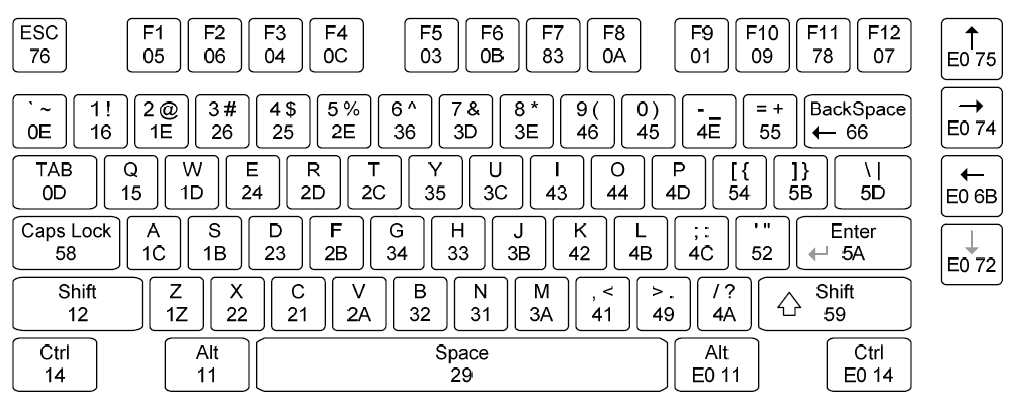
\includegraphics[width=\textwidth]{scancodes.png}
\end{center}
\caption{PS/2 keyboard scan codes}
\label{scancodes}
\end{figure}

Keyboard controller appears to the programmer in memory region
0x1E800000 - 0x1E800FFF. We note that all memory addresses mentioned in this
section are physical addresses. Refer to section \ref{ssec:memman} for
more information on address translation in MIPS architecture. Table
\ref{kbdregs} shows memory-mapped registers of interrupt controller.\\

\begin{figure}[H]
\begin{center}
\begin{tabular}{|c|c|c|c|c|}

\hline \textbf{Memory Address} & \textbf{Access Type} &
       \textbf{Register Name} & \textbf{Function}  \\

\hline 0x1E800000 & READ & KBD\_BUFHEAD & Buffer head register \\
\hline

\end{tabular}
\end{center}
\caption{Keyboard controller registers}
\label{kbdregs}
\end{figure}

It is important to note that all registers are read using
LBU instruction. We summarize the purpose of each
register in the following points:

\begin{itemize}

\item \textbf{KBD\_BUFHEAD}:
A read-only register that is accessed by reading the byte at phsyical
location 0x1E800000. It returns the value of the byte at the head of
the internal buffer. We note that when the buffer head is read,
it is flushed; next read will cause the keyboard controller to return
the next byte in the buffer, and so on, until the buffer becomes empty.
When the buffer is empty, a value of `0' is returned. When ISR executes, the
OS should keep reading this register until it returns zero, to make sure
that all values stored in the buffer are read and no scan code is lost.

\end{itemize}

%------------------------------------------------------------------------------%

\chapter{Implementation}

\section{Overview}

To implement the architecture proposed in the previous chapter, we chose
Nexys II board (from Digilent) which includes a Spartan-3E FPGA chip.
Nexys II is a cheap FPGA board that contains many of the components
we need for our project. Figure \ref{nexys2} shows a photograph
for the PCB board.

\begin{figure}[H]
\begin{center}
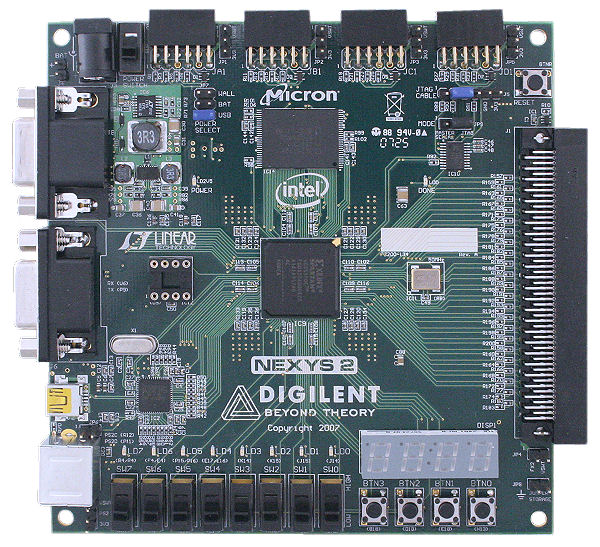
\includegraphics[width=0.8\textwidth]{nexys2.jpg}
\end{center}
\caption{Nexys II board}
\label{nexys2}
\end{figure}

\newpage

The Nexys II PCB board mainly contains the following components:

\begin{itemize}
\item A flash ROM containing our FPGA design.
\item A flash ROM storing our firmware.
\item A pseudo-static RAM to be used by the software to
      store runtime code/data.
\item The FPGA chip itself.
\item A 50MHz crystal oscillator.
\item VGA connector.
\item PS/2 port.
\item USB controller.
\item JTAG logic.
\end{itemize}

We implemented the hardware components (we have described in the architecture
chapter) in VHDL, and compiled the code using Xilinx tools. The output
bitfile is stored in a flash ROM on the board. When the board is powered on,
The FPGA chip is automatically programmed using the bitfile stored on the
ROM, a process that causes our design to be uploaded to the FPGA chip.\\

As we explained in previous chapter, our design consists of a set of
modules (components) that interface each other through a shared system bus.
They also interface the external world (the ROM chip, RAM chip, VGA port,
PS/2 port, and the oscillator) through the pins of the FPGA chip.\\

As we already mentioned before, our design consists of the following
components:

\begin{itemize}

\item \textbf{Central Processing Unit (CPU)}: The core
component of the system, masters the system bus.

\item \textbf{System Bus}: The bus through which all components of the
system inside the FPGA are connected.

\item \textbf{Bus Decoder}: Controls the Chip Select (CS) signals
fed into various I/O devices.

\item \textbf{Memory Interface}:
Interfaces the system bus from one side, and ROM/RAM on-board chips from
the other side.

\item \textbf{VGA Interface}:
Interfaces the system bus from one side, and VGA connector from
the other side.

\item \textbf{Interrupt Controller}:
Works as an interface between the CPU and various interrupt sources.

\item \textbf{Programmable Interval Timer}:
Works as a programmable frequency divider controlled by software.

\item \textbf{Keyboard Controller}:
Interfaces the system bus from one side, and PS/2 port from
the other side.

\end{itemize}

Figure \ref{fpga} shows the organization of those components inside
the FPGA chip, and the connections between them and the outer
world (the chips on the Nexys II board). In next sections, we describe
the implementation of each of the components.

\begin{figure}[H]
\begin{center}
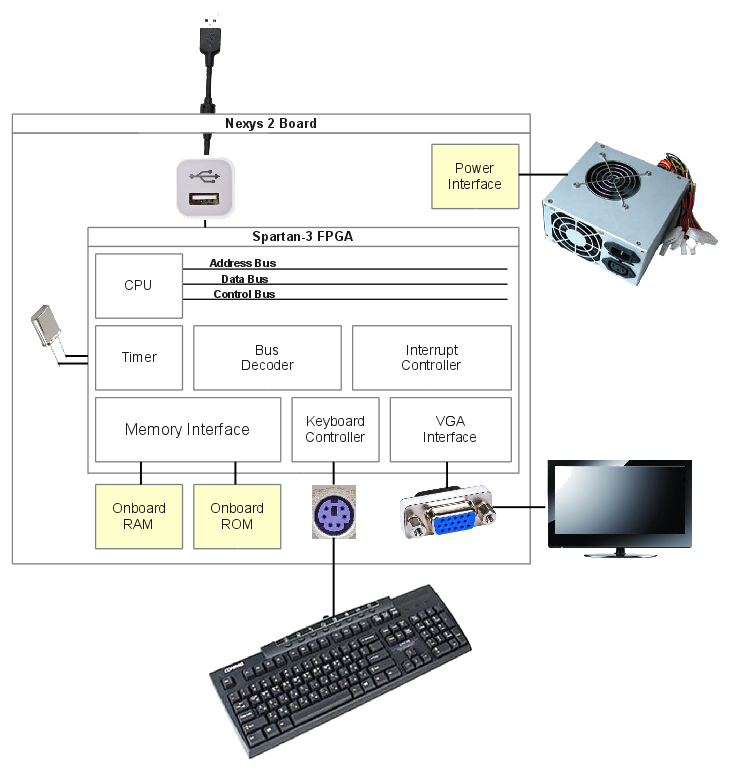
\includegraphics[width=\textwidth]{fpga.png}
\end{center}
\caption{High-level organization of the system}
\label{fpga}
\end{figure}

\newpage

\section {Central Processing Unit}

The CPU core is implemented as a 5-stage pipeline, just like the original
MIPS pipeline, except that the pipeline is extended to implement all the
instructions of MIPS-I instruction set architecture. The five stages are:

\begin{itemize}
\item \textbf{Instruction Fetch (IF)}:
      Responsible for fetching the instructions from instruction cache.
\item \textbf{Instruction Decode (ID)}: Decodes the fetched instruction
      and retrieves values of source registers.
\item \textbf{Execute (EX)}: Executes the instruction.
\item \textbf{Memory (MEM)}: Any data memory read/write is performed here. This
      stage interfaces the data cache.
\item \textbf{Write Back (WB)}: Register write back is performed here.
\end{itemize}

Figure \ref{pipeline}
shows the extended pipeline we created to implement MIPS-I instruction
set architecture. The pipeline also contains a unit for detecting hazards,
and contains forwarding logic as well. The pipeline works under a frequency
of 25MHz (obtained by dividing the 50MHz general clock source by 2). This
was the maximum frequency we could achieve with the Spartan-3E chip.\\

The CPU contains two direct-mapped caches: instruction cache and data cache.
Instructions fetched by IF stage are actually fetched from the instruction
cache. Data read/written by MEM stage are actually read from/written into
data cache. The data cache is write-through cache; any write will cause
the main memory to be updated immediately.\\

A cache miss in any of the caches will cause the pipeline to stall until
data is fetched from/written to the main memory. The caches are implemented
as a separate VHDL module that interfaces the pipeline through an internal
bus. On the other hand, the caches interface the system bus directly.\\

Translation look-aside buffer interfaces the address bus of the IF and MEM
stages with the address bus of the caches. TLB itself is a direct-mapped cache
that stores mappings from virtual page number (VPN) to physical frame numbers
(PFN). A special circuitry handles TLB-related instructions.\\

To summarize, the CPU consists of three basic components: A 5-stage
pipeline, a TLB, and a cache. The three components together interface the main
system bus of the machine.

\begin{figure}[H]
\begin{center}
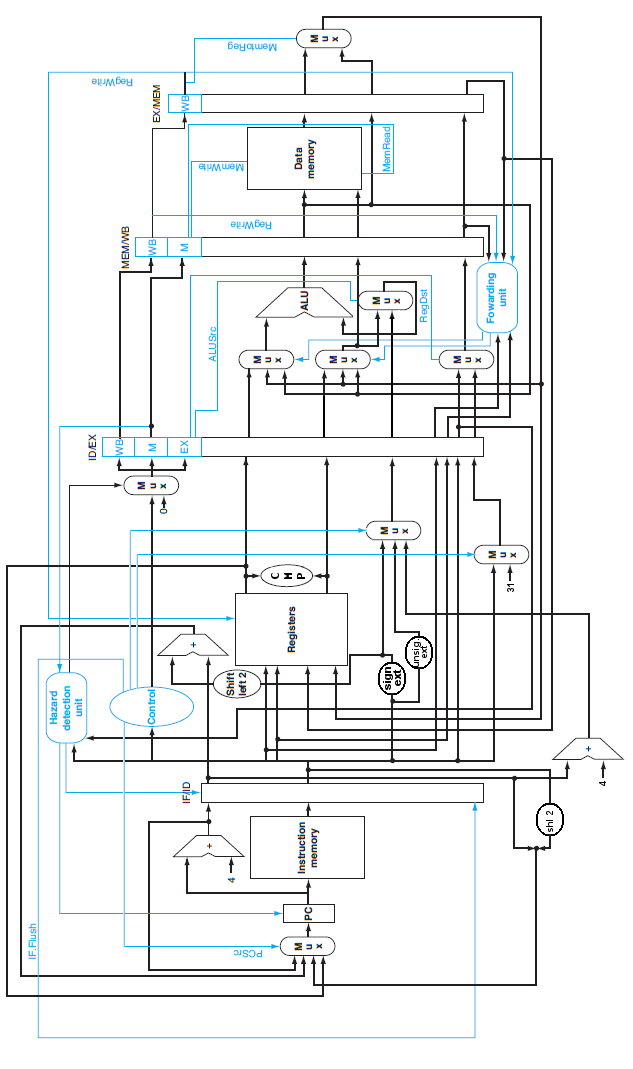
\includegraphics[width=0.85\textwidth]{pipeline.png}
\end{center}
\caption{Our extended MIPS pipeline}
\label{pipeline}
\end{figure}

\section {System Bus}

As we mentioned in the architecture chapter, system bus consists of three
sub-buses: address bus, data bus, and control bus. The address bus is
implemented as 32-bit signal in VHDL, controlled by the CPU and fed into
other components. Because Spartan-3E FPGA doesn't support tri-state buses
inside the FPGA chip, data bus is implemented as several buses:

\begin{itemize}
\item A bus from CPU to other components; used when CPU writes data to
      memory or I/O devices.
\item A bus from each I/O device to the CPU (the buses are OR'd before
      they are fed into the CPU); used when CPU fetches data.
\end{itemize}

Control bus signals are implemented as normal VHDL signals. Chip Select
signals (CS) are controlled by bus decoder and fed into other components.
IRQ\# signals and IAK\# signals interface the interrupt controller with
interrupt sources (VGA and keyboard). IRQ and IAK signals interface
the interrupt controller with CPU.

\section {Bus Decoder}

The bus decoder module simply takes address bus as input and produces
various CS (chip select) signals based on the criteria specified in
architecture chapter. The bus decoder is implemented in VHDL as a
combinational circuit that drives the CS of an I/O device to the
high level if and only if the address lies in its memory region.

\section {Memory Interface}

Nexys II board contains on-board 16MB ROM chip and another 16MB RAM chip.
The two chips are interfaced to the Spartan-3E FPGA chip through a 16-bit
data bus, 24-bit address bus, and a set of control signals as shown
in figure \ref{memory}.\\

The address bus and data bus are shared between the two memory chips.
On the other hand, the MT-CE and ST-CE signals (used to activate/enable
the RAM and ROM, respectively) are separated. It is obvious that
the bus of the memory chips is incompatible with our system bus, therefore
we needed the memory interface component in our design.\\

The memory interface module interfaces our 32-bit system bus with the
external bus shown in figure \ref{memory}. Since RAM and ROM chips data
bus is 16-bit, the memory interface might need to perform two half-word
reads/writes when a 32-bit memory access is issued by the CPU, thus
the memory interface is a sequential circuit.\\

The module takes, as input, CS\_ROM and CS\_RAM signals generated by
bus decoder. If CS\_RAM is activated, the module activates MT-CE
signal (which enables RAM chip). Otherwise, if CS\_ROM signal is
activated, the module activates ST-CE signal, which enables ROM chip.

\begin{figure}[H]
\begin{center}
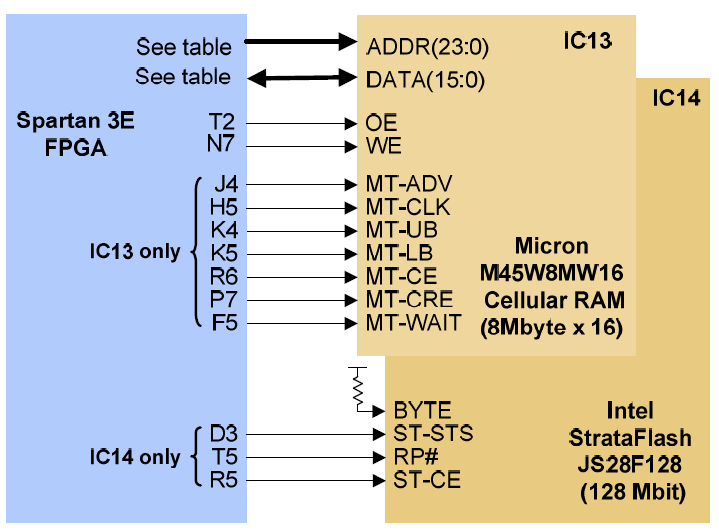
\includegraphics[width=0.85\textwidth]{memory.png}
\end{center}
\caption{Nexys II memory circuits}
\label{memory}
\end{figure}

\section {VGA Interface}

\section {Interrupt Controller}

\section {Programmable Timer}

\section {Keyboard Controller}

%------------------------------------------------------------------------------%

\chapter{Software}

%------------------------------------------------------------------------------%

\chapter{Results}

%------------------------------------------------------------------------------%

\chapter{Conclusion}

\section{Future Work}

%------------------------------------------------------------------------------%

\appendix

\chapter{Instruction Listing}

%------------------------------------------------------------------------------%

%\backmatter

\end{document}
